
\documentclass{report}

\usepackage[utf8]{inputenc}
\usepackage[italian]{babel}
\usepackage{import}
\usepackage{todonotes}
\usepackage{color}
\usepackage{rotating}
\usepackage[hidelinks]{hyperref}
\usepackage{url}
\usepackage{pdfpages}
\usepackage{siunitx}
\usepackage{pdflscape}
\usepackage{subfig}
\usepackage[euler]{textgreek}

\usepackage{enumerate} 
\usepackage{amsmath}
\usepackage{amsfonts}

\usepackage[signatures,swapnames,sans]{frontespizio}

\usepackage{geometry}
\geometry{portrait, margin=3cm}
\usepackage{siunitx}
\usepackage{booktabs}

\renewcommand*\figurename{Figura}

\newcommand{\sub}[1]{\textsubscript{#1}}
\newcommand{\super}[1]{\textsuperscript{#1}}
\newcommand{\parallelsum}{\mathbin{\!/\mkern-5mu/\!}}

\newcommand{\Fig}[0]{Fig.}

\usepackage{titlesec}

\titleformat{\chapter}{\normalfont\huge}{}{20pt}{\huge\bfseries}

\linespread{1.1}

\begin{document}
\addtocounter{chapter}{-1}
	\begin{frontespizio}
		\Margini{3cm}{3cm}{3cm}{3cm}
		\Universita{Bergamo}
		\Logo[43.332mm]{unibg-mark}
		\Divisione{Scuola di Ingegneria}
		\Corso[Laurea Magistrale]{Ingegneria Informatica}
		\Titolo{Elettronica e Misure Industriali}
		\Sottotitolo{Relazione esperienze di laboratorio}
		\Punteggiatura{}
		\NRelatore{Prof.}{Prof.}
		\Relatore{Valerio Re}
		\NCorrelatore{Prof.}{Prof.}
		\Correlatore{Massimo Manghisoni}
		\Candidato[1058231]{Giulia Allievi}
		\Annoaccademico{2021--2022}
		\begin{Preambolo*}
			\usepackage[italian]{babel}
			\usepackage[T1]{fontenc}
			\usepackage[utf8]{inputenc}
			\usepackage{microtype}
			\usepackage{lmodern}
			\graphicspath{{img/}}
			
			\renewcommand{\frontinstitutionfont}{\fontsize{14}{17}\bfseries\scshape}
			\renewcommand{\fronttitlefont}{\fontsize{17}{21}\bfseries\scshape}
			\renewcommand{\frontfootfont}{\fontsize{12}{14}\bfseries\scshape}
		\end{Preambolo*}
	\end{frontespizio}



%----------------------------------------------------------------------------------------
%	PAGINA BIANCA
%----------------------------------------------------------------------------------------
\newpage
\null
\thispagestyle{empty}
\newpage

%----------------------------------------------------------------------------------------
%	INDICE
%----------------------------------------------------------------------------------------
\tableofcontents

%----------------------------------------------------------------------------------------
%	PAGINA BIANCA
%----------------------------------------------------------------------------------------
\newpage
\null
\newpage

%----------------------------------------------------------------------------------------
%	INTRO
%----------------------------------------------------------------------------------------
\chapter{Introduzione}
Nelle esperienze di laboratorio si sono realizzati ed analizzati i seguenti circuiti:
\begin{itemize}
\item Esperienza 1: Emitter follower con alimentazione duale; 
\item Esperienza 2: Emitter follower con alimentazione singola; 
\item Esperienza 3: Common emitter amplifier con alimentazione duale e singola; 
\item Esperienza 4: Amplificatore invertente ed integratore con 	\textmu A741.
\end{itemize}
La relazione è suddivisa per tipologia di circuito.
%----------------------------------------------------------------------------------------
%	CIRCUITO 1: EMITTER FOLLOWER	
%----------------------------------------------------------------------------------------
\chapter{Circuito 1: Emitter Follower}
\section{Introduzione} \label{introEFv1}
Il primo circuito realizzato è l'\textit{Emitter follower}, detto anche \textit{Common collector}. Questo circuito ha un guadagno unitario, infatti la tensione misurata in uscita è uguale alla tensione applicata in ingresso, perciò si comporta come un buffer. Ne abbiamo realizzate due diverse versioni, una con alimentazione duale ed una con alimentazione singola. 
\section{Prima versione} % alimentazione duale
La prima versione di \textit{Emitter follower} analizzata è quella ad alimentazione duale. Di seguito si riportano lo schema (figura \ref{figura:EFv1}), l'analisi del punto di lavoro e di piccolo segnale, e le misure effettuate su questo circuito. 
\begin{figure}[h]
\centering
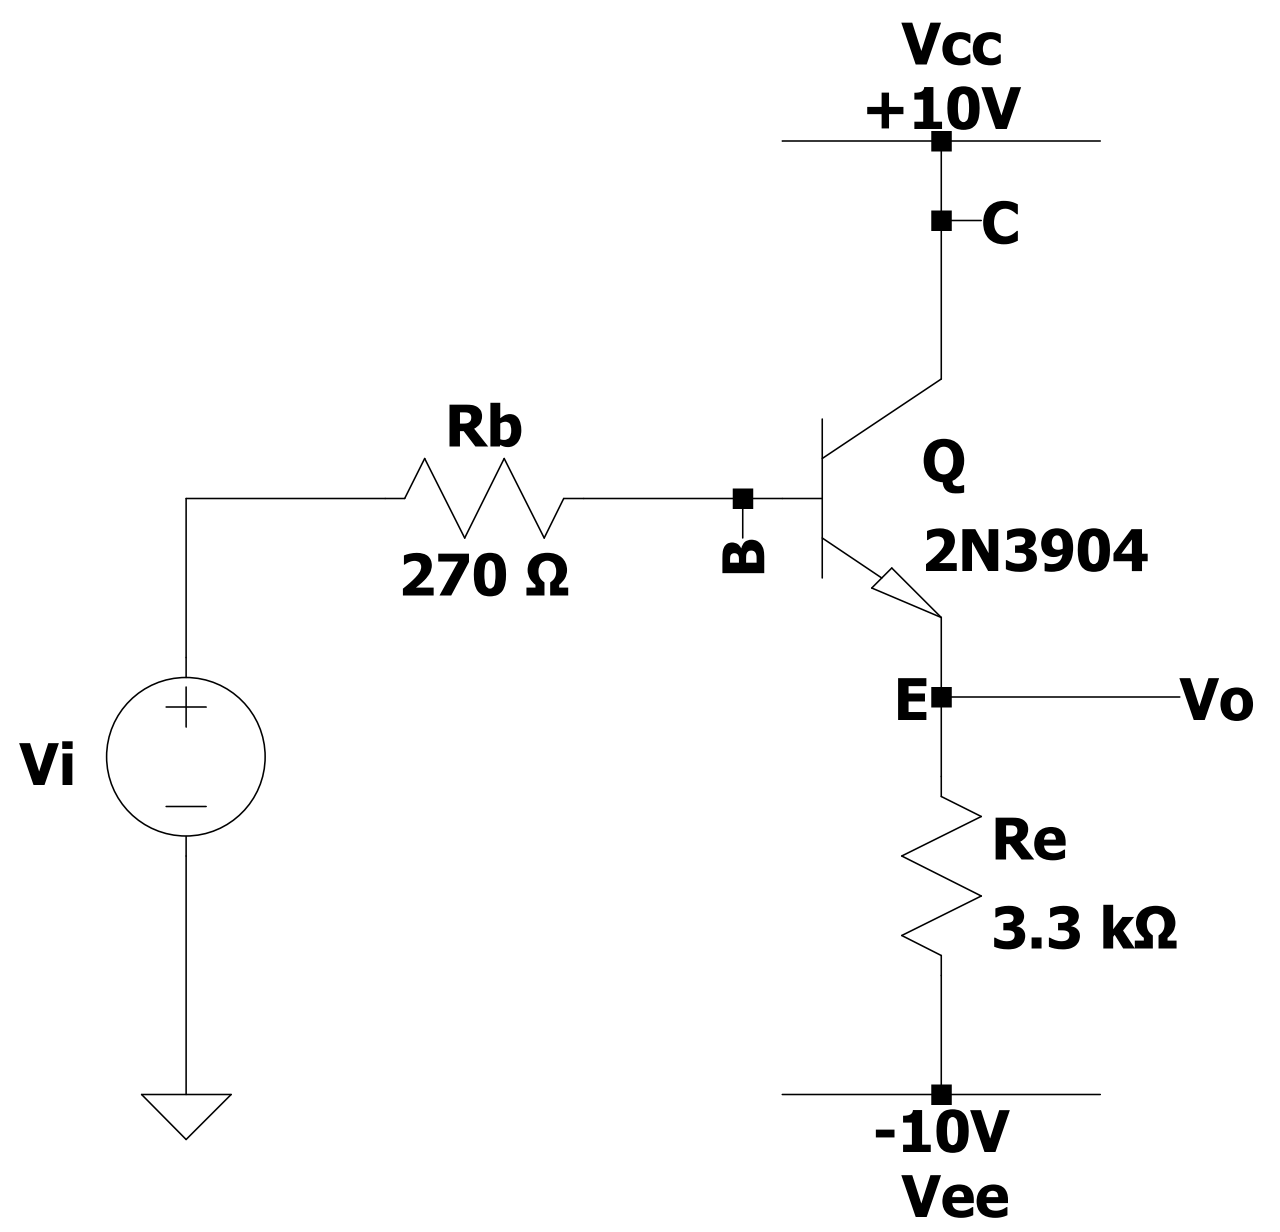
\includegraphics[height=10cm]{immagini/EFv1}
\caption{Schema dell'\textit{Emitter follower} ad alimentazione duale.}
\label{figura:EFv1}
\end{figure}
\subsection{Punto di lavoro} \label{puntolavoroEFv1}
In quest'analisi bisogna spegnere i generatori di segnale e sostituirli con un cortocircuito se sono generatori di tensione, oppure con un circuito aperto se sono generatori di corrente. I condensatori sono sostituiti con un circuito aperto e gli induttori con un cortocircuito. Successivamente si va a determinare la tensione di ogni nodo e la corrente che scorre in ogni ramo. 
\begin{figure}[h]
\centering
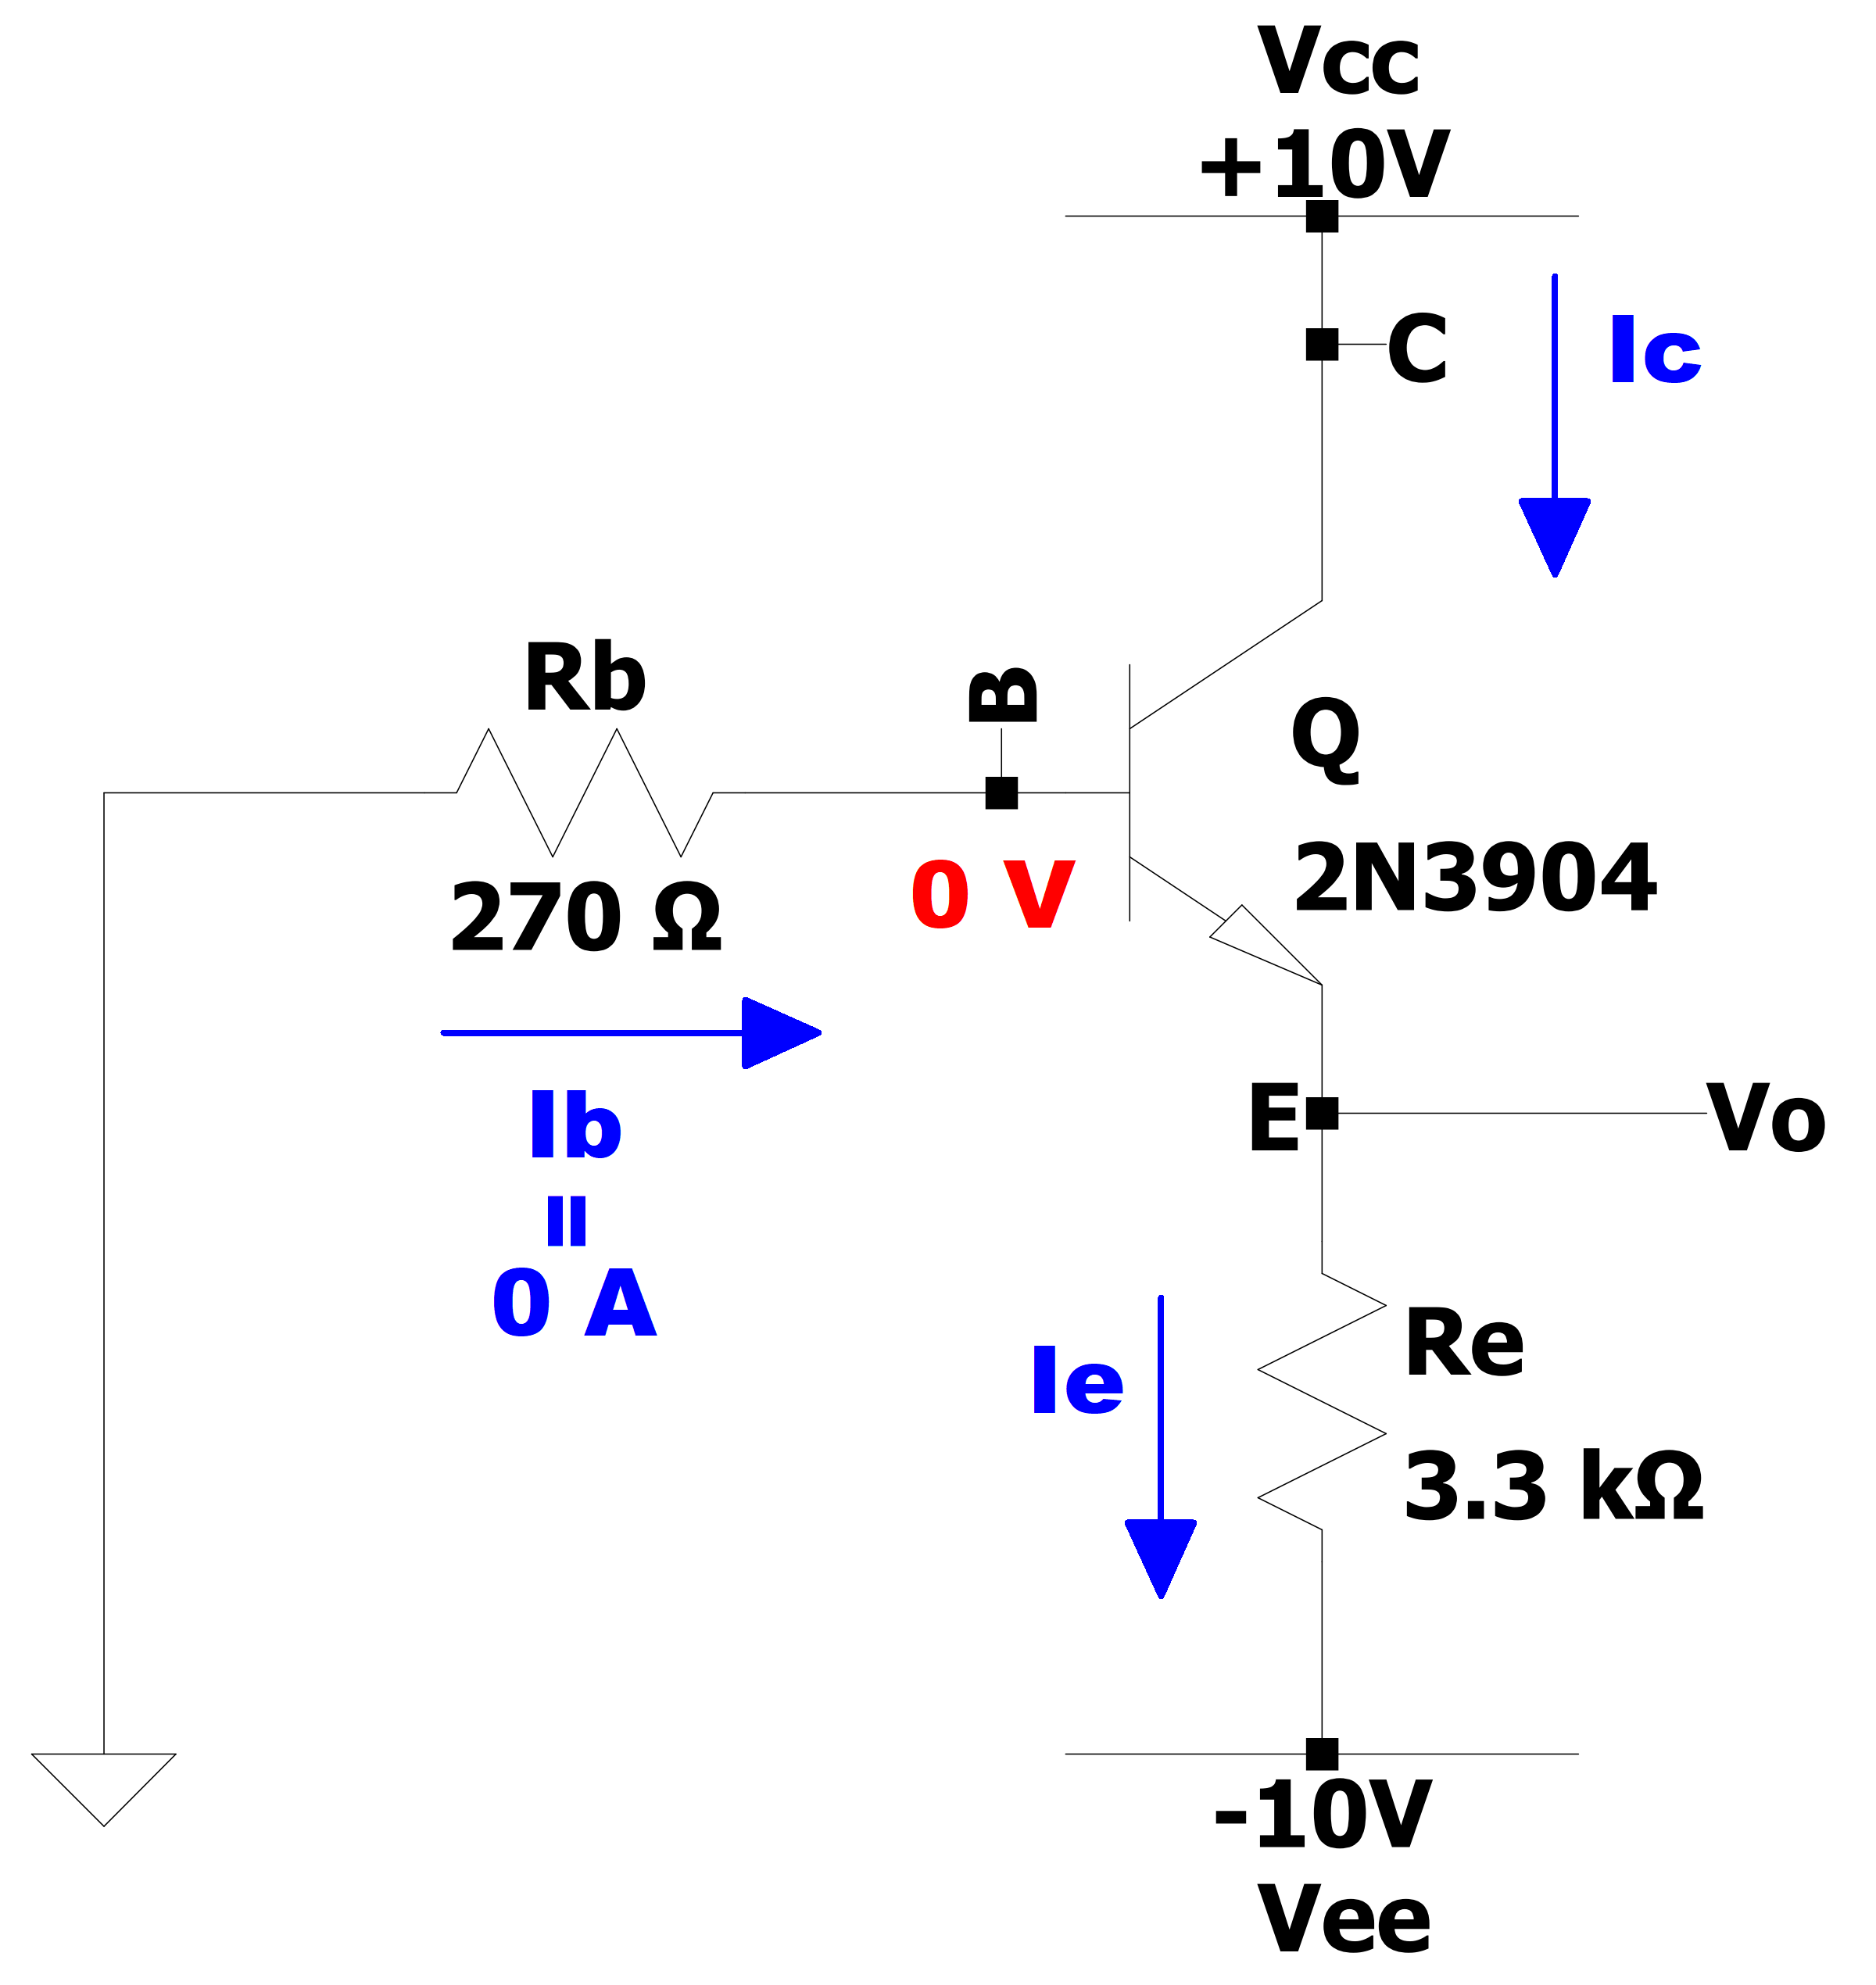
\includegraphics[height=10cm]{immagini/EFv1_pl}
\caption{Punto di lavoro dell'\textit{Emitter follower} ad alimentazione duale.}
\label{figura:EFv1_pl}
\end{figure}
\\Come si vede nell'immagine~\ref{figura:EFv1_pl}, il generatore di segnale $v_{i}$ viene sostituito con un cortocircuito, quindi la resistenza $R_{B}$ si trova fra massa e la base del transistor \textit{Q}. In questo caso non dobbiamo apportare altre modifiche al circuito originale. 
\\Nell'analisi utilizziamo il modello ideale del transistor, perciò assumiamo che $\displaystyle{\beta\rightarrow\infty}$ e che $I_{B}=0A$, di conseguenza la corrente che fluisce nella resistenza è nulla, perciò, per la legge di Ohm, sarà nulla anche la caduta di tensione ai suoi capi, quindi si ricava che $V_{B}=0V$. 
\\Dal bilancio di correnti del  transistor (lo trattiamo come se fosse un nodo) otteniamo che $I_C+I_B=I_E$, ma dato che $I_{B}$ è nulla, allora $I_C=I_E$.
\\Suppondendo che il transistor si trovi in regione attiva diretta, la tensione $V_{BE}$ fra la base e l'emettitore è pari a circa +0.7V perché la giunzione è polarizzata direttamente. Dato che sappiamo che $V_{B}=0V$, possiamo calcolare per differenza $V_{E}$, dunque $V_{E}=0V-0.7V=-0.7V$. Anche $V_o$ sarà pari a questo valore dato che l'uscita viene prelevata all'emettitore.
\\$V_C$ è pari alla tensione di alimentazione positiva, perciò $V_C=V_{CC}=10V$.
Dato che $V_{CB}>0V$, la giunzione base-collettore è polarizzata inversamente, quindi l'ipotesi che il transistor si trovi in regione attiva diretta è verificata. 
\\Ora possiamo calcolare la corrente di emettitore con la legge di Ohm: 
\\[2pt]\indent$\displaystyle{V_E-V_{EE}=R_E\cdot I_E \rightarrow I_E=I_C=\frac{V_E-V_{EE}}{R_E}=\frac{-0.7V-(-10V)}{3.3k\Omega}=2.818mA}$
\\[2pt]Il circuito è ora completamente risolto, come ultima cosa si può calcolare la transconduttanza, visto che ci servirà successivamente per l'analisi di piccolo segnale. La transconduttanza è definita come il rapporto tra la corrente di collettore stazionaria $I_C$ e la tensione termica $V_T$, che a temperatura ambiente vale circa 26mV. 
\\[2pt]In formule: $\displaystyle{g_m=\frac{I_C}{V_T}=\frac{2.818mA}{26mV}=0.108 \frac{A}{V}}$.
\\[3pt]In tabella \ref{table:EFv1_pl} sono riassunte tutte le grandezze ricavate dal punto di lavoro. 
\begin{table}[h]
	\centering
	\begin{tabular}{|c|c|c|c|c|c|c|}
		\hline
		\textbf{V\ped{B}[V]} & \textbf{V\ped{C}[V]} & \textbf{V\ped{E}[V]} & \textbf{I\ped{B}[A]} & \textbf{I\ped{E}[mA]} & \textbf{I\ped{C}[mA]} & \textbf{g\ped{m}[A/V]} \\ 
		\hline
		0 & 10 & -0.7 & 0 & 2.818 & 2.818 & 0.108\\ 
		\hline
	\end{tabular}
\caption{Riassunto delle grandezze ricavate dal punto di lavoro del circuito.}
\label{table:EFv1_pl}
\end{table}
\subsection{Analisi di piccolo segnale} \label{piccolosegnaleEFv1}
Nell'analisi di piccolo segnale bisogna spegnere i generatori di grandezze continue e sostituirli con un cortocircuito se sono generatori di tensione, oppure con un circuito aperto se sono generatori di corrente. Per analisi approssimate, i condensatori sono sostituiti con un cortocircuito e gli induttori con un circuito aperto; per analisi più accurate, invece, non vengono sostituiti e si utilizza la loro impedenza per risolvere il circuito. Infine, i transistor vengono sostituiti con il loro modello per piccolo segnale. Successivamente si va a determinare la tensione di ogni nodo e la corrente che scorre in ogni ramo, esattamente come avveniva per l'analisi del punto di lavoro. 
\begin{figure}[h]
\centering
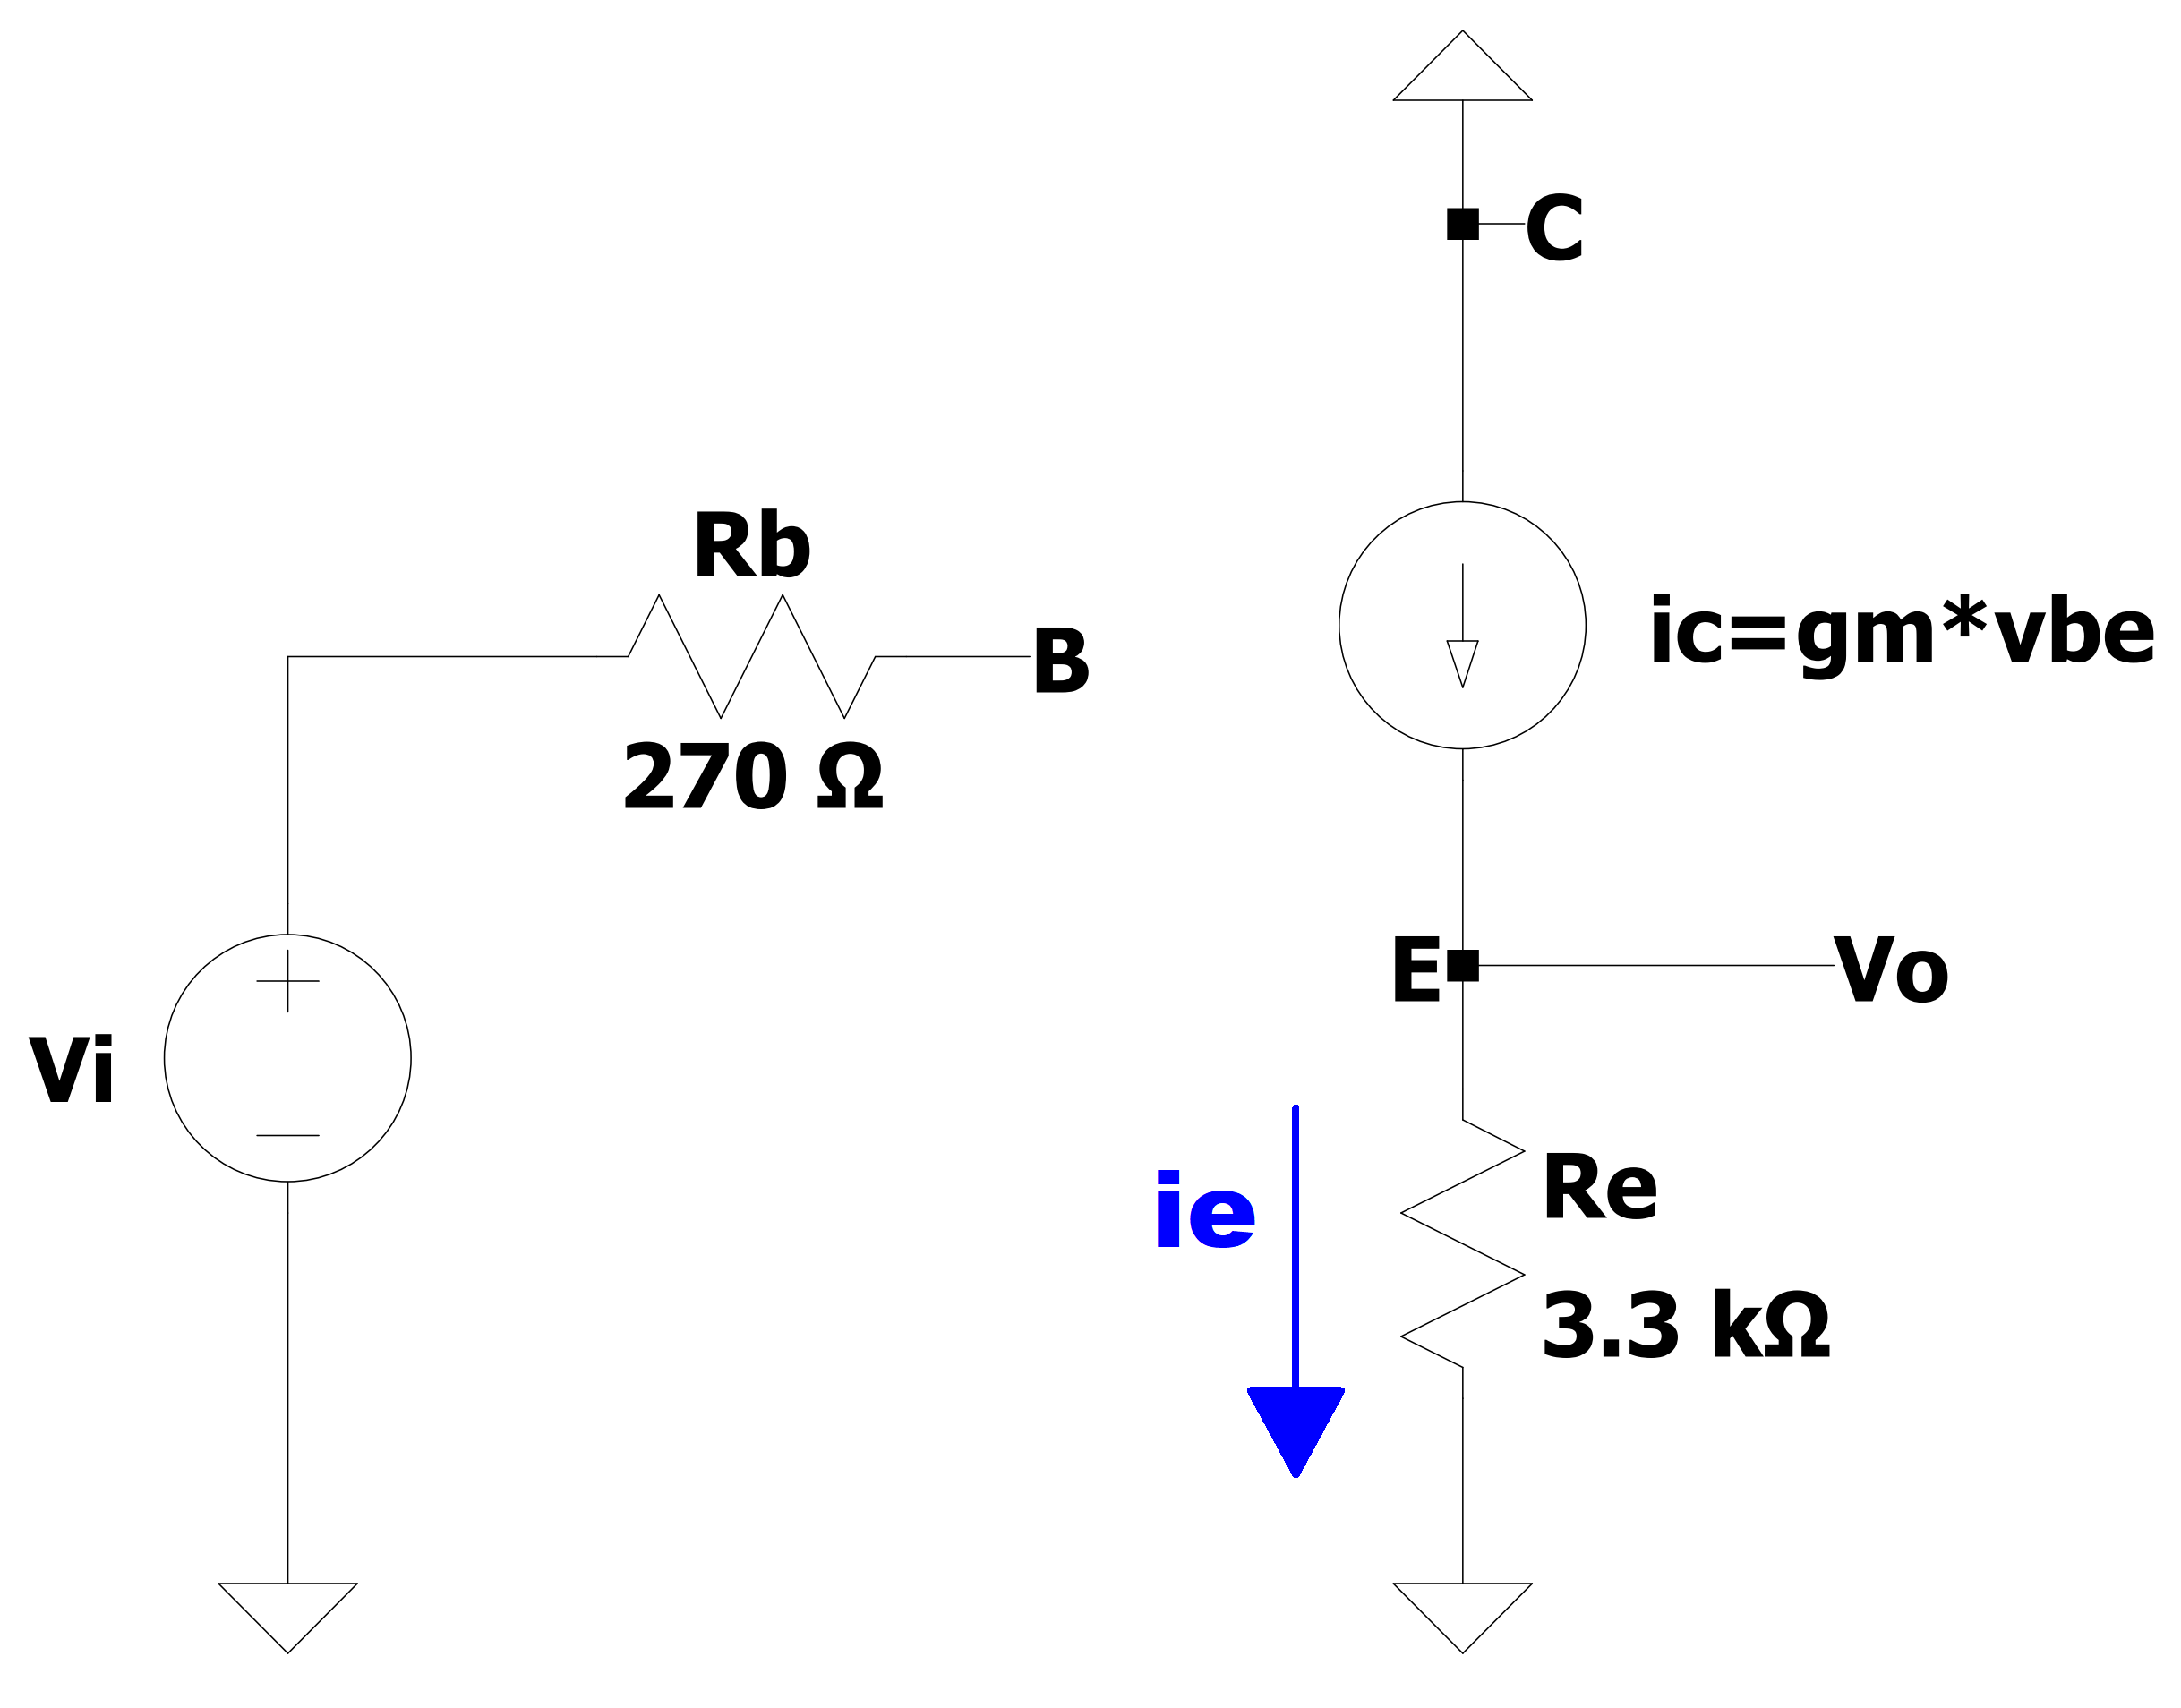
\includegraphics[height=9.6cm]{immagini/EFv1_ps}
\caption{Analisi di piccolo segnale dell'\textit{Emitter follower} ad alimentazione duale.}
\label{figura:EFv1_ps}
\end{figure}
\\Come si può notare dalla figura~\ref{figura:EFv1_ps}, il BJT viene sostituito con il modello per piccolo segnale a bassa frequenza, quindi il terminale di base risulta isolato dal collettore e dall'emettitore; invece, questi due terminali sono collegati attraverso un generatore di corrente ideale di valore pari al prodotto fra la transconduttanza $g_m$ e la tensione $v_{BE}$.
\\Dato che la base del transistor è isolata, nel circuito di sinistra non circola corrente, perciò non c'è caduta di tensione sulla resistenza $R_B$, quindi la tensione $v_B$ risulta pari alla tensione applicata in ingresso con il generatore $v_i$.
\\Abbiamo già detto che $i_C=g_m\cdot v_{BE} = g_m(v_B-v_E) $. Ma dato che $v_B=v_i$ e $v_E=v_o$, la formula precedente per il calcolo della corrente di collettore si può riscrivere come $i_C=g_m(v_i-v_o)$.
\\[2pt]Ricaviamo $i_E$ con la legge di Ohm: 
$\displaystyle{i_E=\frac{v_E-0V}{R_E}=\frac{v_o}{R_E}}$.
\\[2 pt] Dal bilancio delle correnti al nodo E otteniamo che $i_C=i_E$. Sostituendo alle due correnti le espressioni ricavate ai punti precedenti possiamo scrivere la seguente eqauazione:
\\[2pt]\indent $\displaystyle{g_m(v_i-v_o)=\frac{v_o}{R_E}}$.
\\[2pt] A questo punto possiamo ricavare la funzione di trasferimento del circuito manipolando l'espressione ottenuta in precedenza. Questa risulta:
\\[2pt]\indent $\displaystyle{\frac{v_o}{v_i}=\frac{g_mR_E}{1+g_mR_E}\simeq1}$ per $g_mR_E\gg 1$. 
\\[2pt]Allora, si può dire che $v_o=v_i$, ovvero il circuito si comporta come un buffer, come si era già accennato nell'introduzione del circuito (sezione \ref{introEFv1}).
\subsection{Componenti, strumenti e misure} 
Il circuito, mostrato in figura \ref{figura:fotoEFv1}, è stato realizzato su una breadboard utilizzando questi componenti:
\begin{itemize}
\item transistor bipolare NPN 2N3904;
\item una resistenza da \SI{270}{\ohm} per $R_B$;
\item due resistenze, una da \SI{1.5}{k\ohm} ($R_{E_1}$) ed una da \SI{1.8}{k\ohm} ($R_{E_2}$) connesse in serie, per realizzare la resistenza $R_E$ da \SI{3.3}{k\ohm}.
\end{itemize}
\begin{figure}[h]
\centering
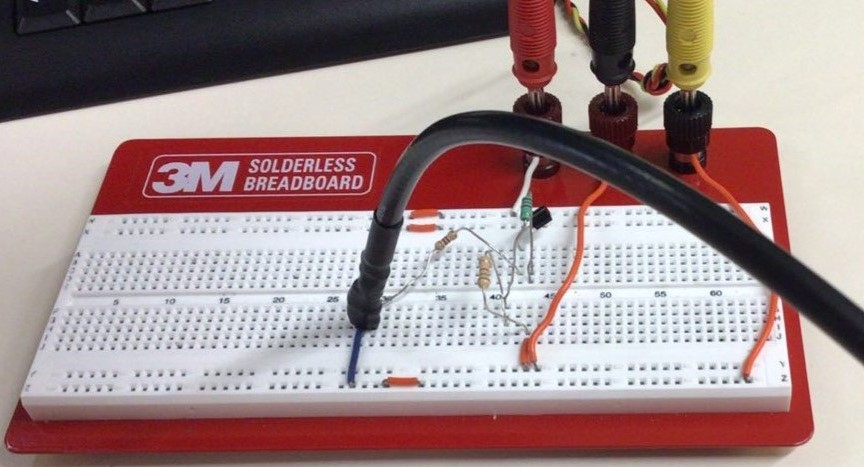
\includegraphics[height=6.6cm]{immagini/fotoEFv1}
\caption{Fotografia del circuito \textit{Emitter follower} ad alimentazione duale realizzato in laboratorio.}
\label{figura:fotoEFv1}
\end{figure}
Per le misure e le analisi, sono stati utilizzati i seguenti strumenti:
\begin{itemize}
\item alimentatore da banco, con alimentazione positiva impostata a 10V ed alimentazione negativa a -10V, entrambe con limite in corrente di 50mA;
\item generatore di forme d'onda;
\item multimetro da banco;
\item oscilloscopio a due canali.
\end{itemize}
Per prima cosa, con il multimetro si sono misurati i valori delle resistenze ed i valori delle tensioni delle giunzioni p-n del transistor (tensione \textit{base-emettitore} e tensione \textit{base-collettore}). I valori ottenuti sono mostrati in tabella \ref{table:EFv1_comp}.
\begin{table}[h]
	\centering
	\begin{tabular}{|c|c|c|}
	\cline{2-3} 
	\multicolumn{1}{c|}{} & \textbf{Valore nominale} & \textbf{Valore misurato}\\ 
		%\hline
		%{} & \textbf{Valore nominale} & \textbf{Valore misurato} \\ 
		\hline
		$\mathbf{R_B}$ & \SI{270}{\ohm} & \SI{271}{\ohm} \\ 
		\hline
		$\mathbf{R_{E_1}}$& \SI{1.5}{k\ohm} & \SI{1.448}{k\ohm} \\ 
		\hline
		$\mathbf{R_{E_2}}$& \SI{1.8}{k\ohm} & \SI{1.788}{k\ohm} \\ 
		\hline
		$\mathbf{V_{BE}}$& $\mathrm{ \simeq0.7V}$ & 0.699V \\ 
		\hline
		$\mathbf{V_{BC}}$& $\mathrm{ \simeq0.7V}$  & 0.659V \\ 
		\hline
	\end{tabular}
	
\caption{Grandezze misurate prima di realizzare il circuito.}
\label{table:EFv1_comp}
\end{table}
\\Le due giunzioni p-n hanno valori di tensione diversi, questo è dovuto alla tecnologia di realizzazione del BJT: essendo un dispositivo planare, le due giunzioni hanno lunghezza diversa, di conseguenza anche il loro valore di tensione sarà diverso. Il valore totale della resistenza $R_E$ è pari a \SI{3.236}{k\ohm}, poco meno del 2\% rispetto al suo valore nominale che è \SI{3.3}{k\ohm}.
\\\indent Dopo aver posizionato tutti i componenti sulla breadboard, è stato fatto lo studio del punto di lavoro del circuito. Non è stato applicato il segnale e il terminale della resistenza $R_B$ non connesso alla base del transistor è stato collegato a massa. Il circuito risultante è mostrato in figura \ref{figura:fotoEFv1_pl}.
\begin{figure}[h]
\centering
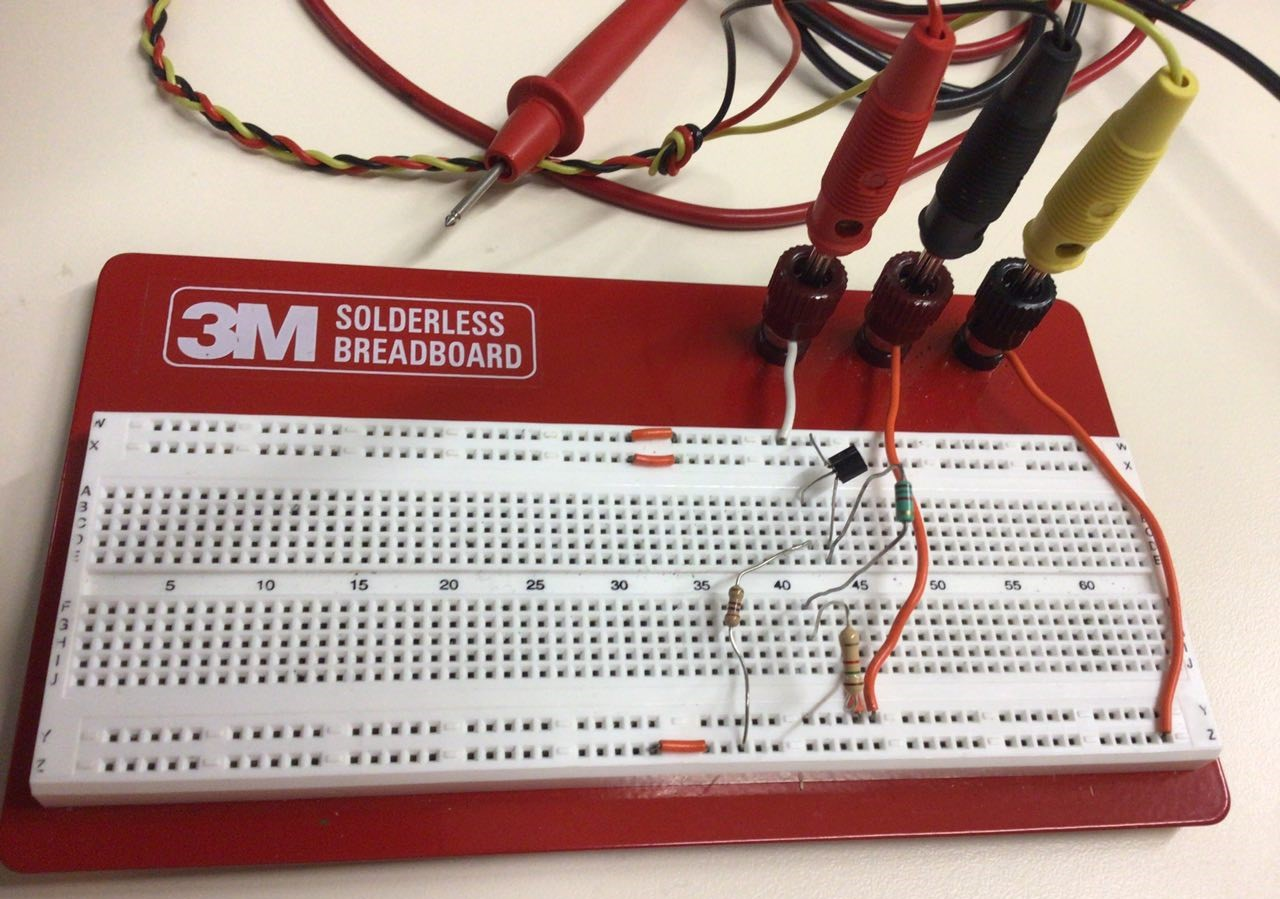
\includegraphics[height=7.3cm]{immagini/fotoEFv1_pl}
\caption{Fotografia del circuito \textit{Emitter follower} con le connessioni per lo studio del punto di lavoro.}
\label{figura:fotoEFv1_pl}
\end{figure}
\\Le tensioni sono state misurate con il multimetro da banco, le correnti di base e di emettitore sono state ricavate utilizzando la legge di Ohm, mentre la corrente di collettore è stata calcolata per differenza dalle altre due correnti. I risultati sono mostrati in tabella \ref{table:EFv1_pl_mis}. 
\begin{table}[h]
	\centering
	\begin{tabular}{|c|c|c|c|c|c|c|}
		\hline
		\textbf{V\ped{B}[mV]} & \textbf{V\ped{C}[V]} & \textbf{V\ped{E}[V]} & \textbf{I\ped{B}[mA]} & \textbf{I\ped{E}[mA]} & \textbf{I\ped{C}[mA]} & \textbf{g\ped{m}[A/V]} \\ 
		\hline
		-3.515 & 10.000 & -0.687 & 0.013 & 2.878 & 2.865 & 0.108\\ 
		\hline
	\end{tabular}
\caption{Grandezze misurate dallo studio del punto di lavoro del circuito.}
\label{table:EFv1_pl_mis}
\end{table}
\\I valori ottenuti sono confrontabili con i risultati teorici calcolati nella sezione \ref{puntolavoroEFv1}. La differenza principale è che sia $V_B$ che $I_B$ non sono nulle, anche se il loro valore (in modulo) è molto piccolo. In particolare, dato che la corrente $I_B$ è piccola, l'approssimazione adottata nello studio teorico del circuito di trascurarla è ragionevole. 
\\\indent Dopo lo studio del punto di lavoro del circuito, è stato applicato in ingresso il segnale collegando con un cavo BNC il generatore di forme d'onda al circuito. Il circuito risultante è quello già mostrato in figura \ref{figura:fotoEFv1}. La forma d'onda utilizzata è una sinusoide con tensione picco-picco $V_{PP}$ di 2V e frequenza $f$ pari a \SI{1}{k\hertz}. 
\\\indent Per visualizzare graficamente la tensione in ingresso e la tensione in uscita è stato utilizzato l'oscilloscopio. Entrambe le sonde sono state collegate a massa con il coccodrillo, la punta di una sonda è stata collegata alla base del transistor (canale 1, traccia gialla) mentre la punta dell'altra sonda è stata collegata all'emettitore (canale 2, traccia azzurra). Il grafico è visibile in figura \ref{figura:oscillo1}.
\begin{figure}[h]
\centering
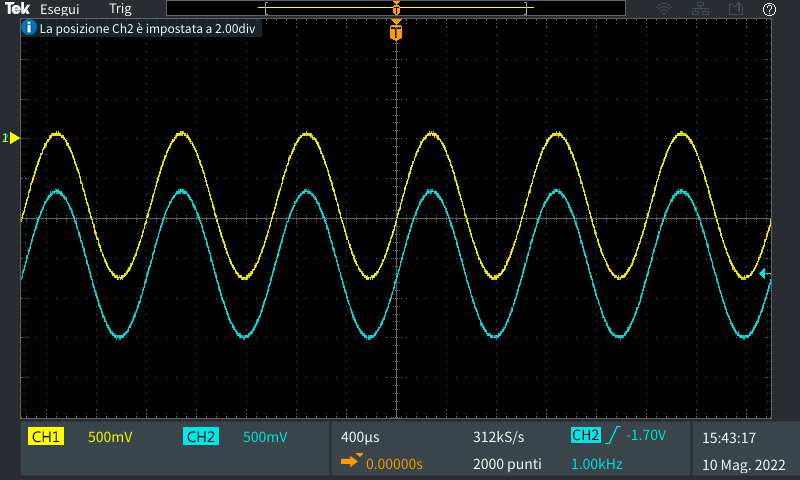
\includegraphics[height=7cm]{immagini/oscillo1}
\caption{Grafico della tensione in ingresso (CH1) e della tensione in uscita (CH2) al circuito.}
\label{figura:oscillo1}
\end{figure}
\\
Com'è possibile vedere dal grafico, il guadagno del circuito è unitario perché entrambe le sinusoidi hanno la stessa ampiezza. La tensione applicata in ingresso la misuriamo in uscita con una differenza di circa 0.7V, che è la caduta di tensione data dalla giunzione p-n fra base ed emettitore. I due segnali sono in fase. 
\\\indent In realtà, il guadagno del circuito non è esattamente unitario e nemmeno lo sfasamento, o offset, è proprio nullo, come invece sembrerebbe dal grafico precedente. La tensione in uscita è legata alla tensione in ingresso da una relazione del tipo $y=a+bx$, dove $y$ è la tensione in uscita, $x$ la tensione in ingresso, $a$ l'offset e $b$ il guadagno del circuito. Per ricavare il valore dei parametri $a$ e $b$ sono state applicate in ingresso al circuito diverse sinusoidi, tutte di frequenza \SI {1}{k\hertz} ma di ampiezza variabile. La tensione picco-picco è infatti stata variare da 0.5V a 5.0V con step di 0.5V. Successivamente, con l'oscilloscopio, si sono misurati i valori di tensione picco-picco in ingresso, $V_{PP_i}$, e in uscita, $V_{PP_o}$. 
\\\indent Per ridurre l'effetto dei disturbi e del rumore sulle misure, i segnali sono stati filtrati con un passa-basso con frequenza di taglio di \SI{20}{M\hertz}, poi sono stati mediati utilizzando 16 acquisizioni. Facendo così, il valore misurato dall'oscilloscopio risulta molto più stabile. Le misure sono riportate in tabella \ref{table:tabgrafico}.
\begin{table}[h]
	\centering
	\begin{tabular}{|c|c|}
		\hline
		$\mathbf{V_{PP_i}[V]}$ & $\mathbf{V_{PP_o}[V]}$\\ 
		\hline
		0.503 & 0.505 \\
		\hline
		1.000 & 1.006 \\
		\hline
		1.497 & 1.506 \\
		\hline
		1.989 & 2.002 \\
		\hline
		2.486 & 2.502 \\
		\hline
		2.978 & 3.001 \\
		\hline
		3.473 & 3.496 \\
		\hline
		3.965 & 3.993 \\
		\hline
		4.461 & 4.497 \\
		\hline
		4.951 & 4.985 \\
		\hline
	\end{tabular}
\caption{Valori della tensione picco-picco in ingresso e in uscita al circuito.}
\label{table:tabgrafico}
\end{table}
\\I dati della tabella precedente sono stati elaborati su MATLAB per ricavare la retta di regressione che ci permette di stimare i valori di $a$ e $b$. Nel grafico seguente, la figura \ref{figura:graficoEFv1}, si riportano le misure, la retta interpolata e la retta teorica. 
\begin{figure}[h]
\centering
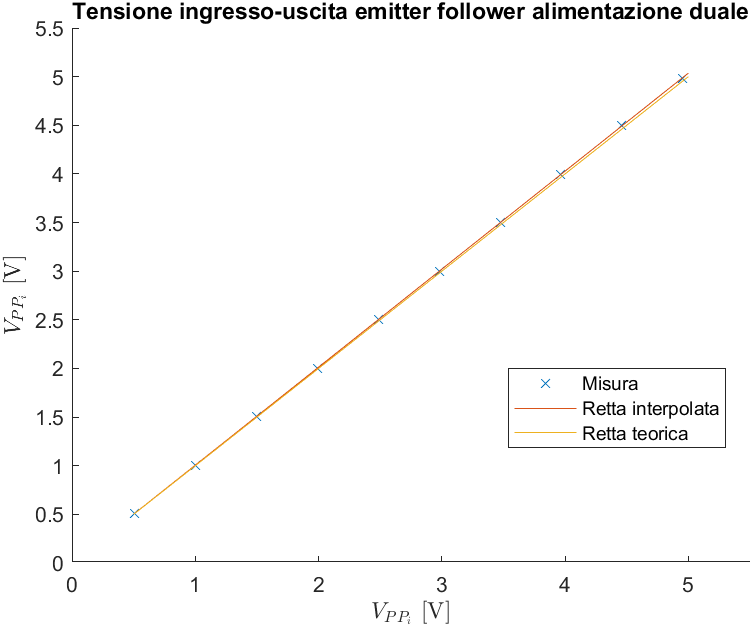
\includegraphics[height=7cm]{immagini/graficoEFv1}
\caption{Confronto grafico fra la tensione ingresso-uscita interpolata e quella teorica.}
\label{figura:graficoEFv1}
\end{figure}
\\L'equazione della retta interpolata è: $y=-0.0020949+1.0077x$. Il risultato è chiaramente in disaccordo con la teoria, perché sebbene il guadagno è molto prossimo all'unità, non può essere maggiore, perché questo significherebbe che il circuito eroga più energia rispetto a quella fornita in ingresso. \\\\ Infatti, il circuito ha una resistenza d'uscita $r_{out}$ di valore circa pari a:
\\[2pt]\indent$\displaystyle{r_{out}\simeq\frac{1}{g_m}}$ \indent con  $\displaystyle{g_m=\frac{I_C}{V_T}}$
\\[2pt]La funzione di trasferimento di conseguenza è leggermente diversa da quella ottenuta alla fine della sezione \ref{piccolosegnaleEFv1}, ed è uguale a:
\\[2pt]\indent $\displaystyle{\frac{v_o}{v_i}=\frac{R_E}{r_{out}+R_E}}$
\\[2pt]da cui risulta evidente che il guadagno non può essere sicuramente maggiore di uno. Il motivo di questo risultato anomalo può essere dovuto alla regolazione non sufficientemente precisa della capacità di compensazione della sonda collegata al secondo canale dell'oscilloscopio.
\section{Seconda versione} % alimentazione singola
Nel circuito appena realizzato abbiamo usato due alimentazioni, una positiva ed una negativa. Se il circuito non fosse alimentato con l'alimentatore da banco, per farlo funzionare servirebbero due batterie da 10V. Adottando alcuni accorgimenti, si può modificare il circuito discusso prima per fare in modo che funzioni con una sola alimentazione, l'altra viene collegata a massa. Siamo perciò passati a studiare l'\textit{Emitter follower} ad alimentazione singola. Il circuito di partenza è mostrato in figura \ref{figura:EFv2_1}, è lo stesso circuito di figura \ref{figura:EFv1} ma al posto dell'alimentazione negativa troviamo la massa. Trascuriamo per ora i valori delle resistenze. Verrano man mano discusse le modifiche e le eventuali problematiche che si riscontreranno per arrivare alla versione finale del circuito.
\begin{figure}[h]
\centering
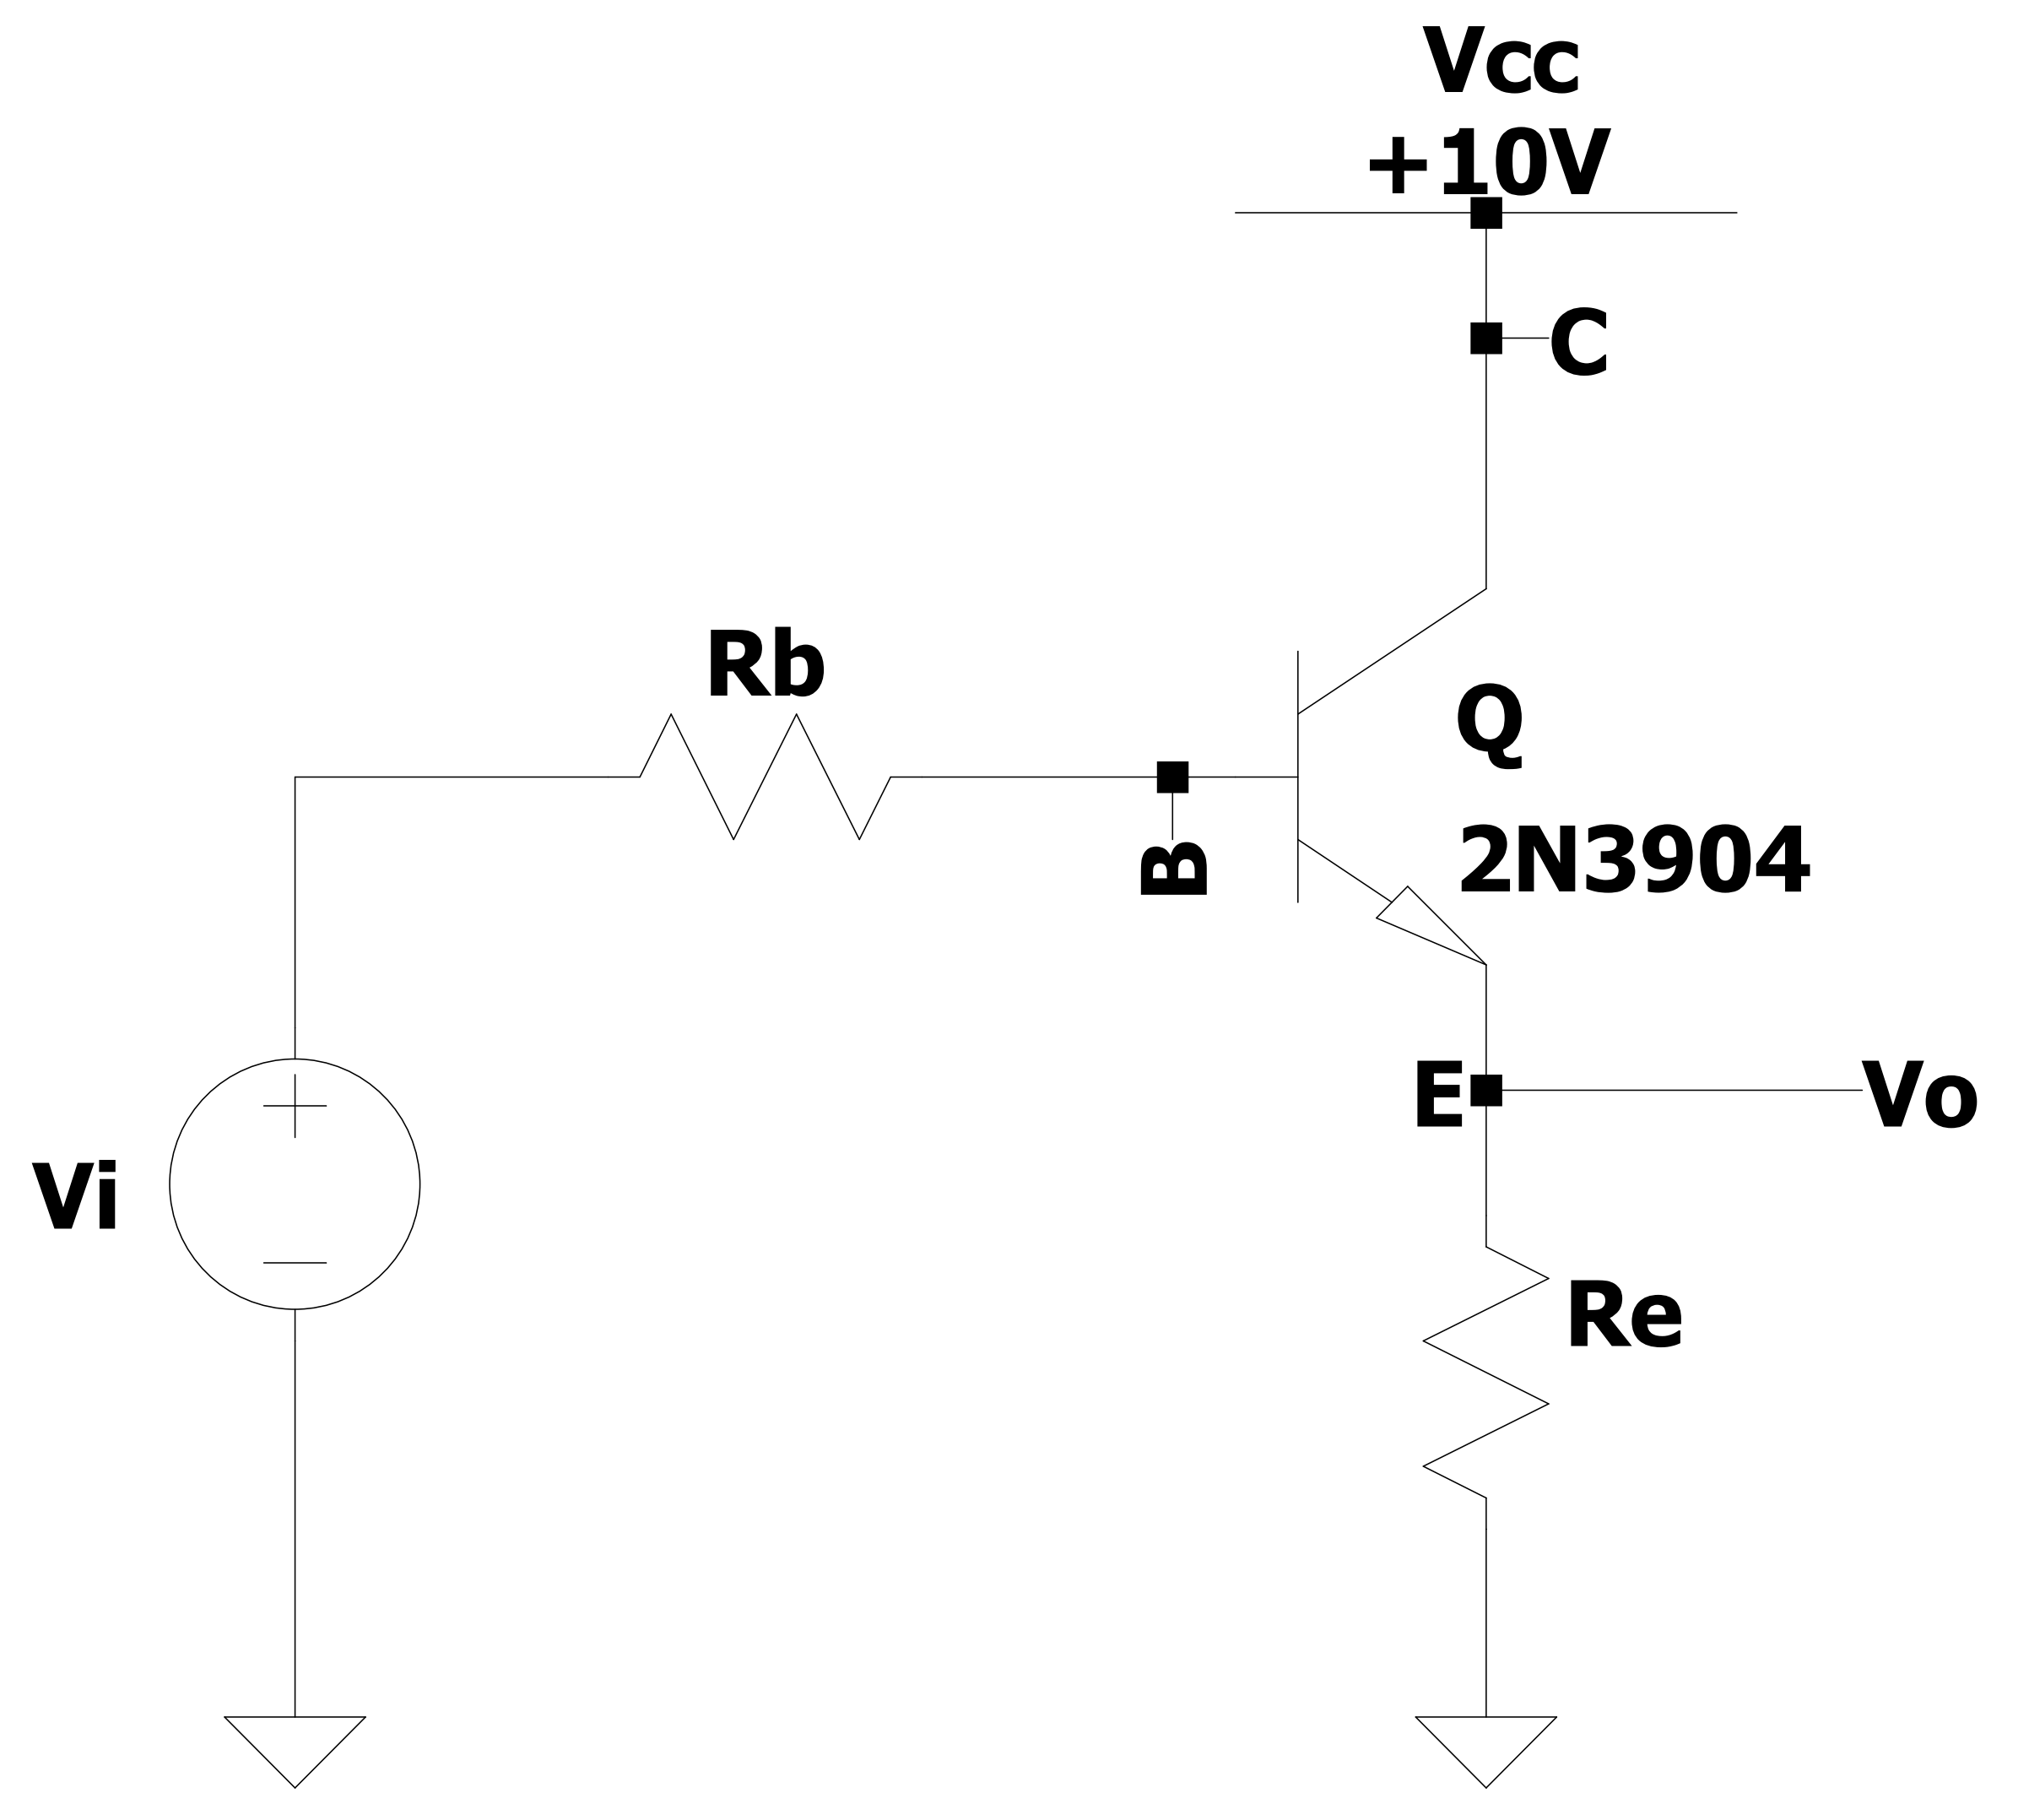
\includegraphics[height=10cm]{immagini/EFv2_1}
\caption{Schema di partenza dell'\textit{Emitter follower} ad alimentazione singola.}
\label{figura:EFv2_1}
\end{figure}
\subsection{Punto di lavoro} % versione base + versione partitore + versione condensatore
Per quest'analisi è sufficiente sostituire il generatore di tensione $v_i$ con un cortocircuito, esattamente come per l'\textit{Emitter follower} ad alimentazione duale. Lo schema risultante è riportato in figura \ref{figura:EFv2_1_pl}.
\begin{figure}[h]
\centering
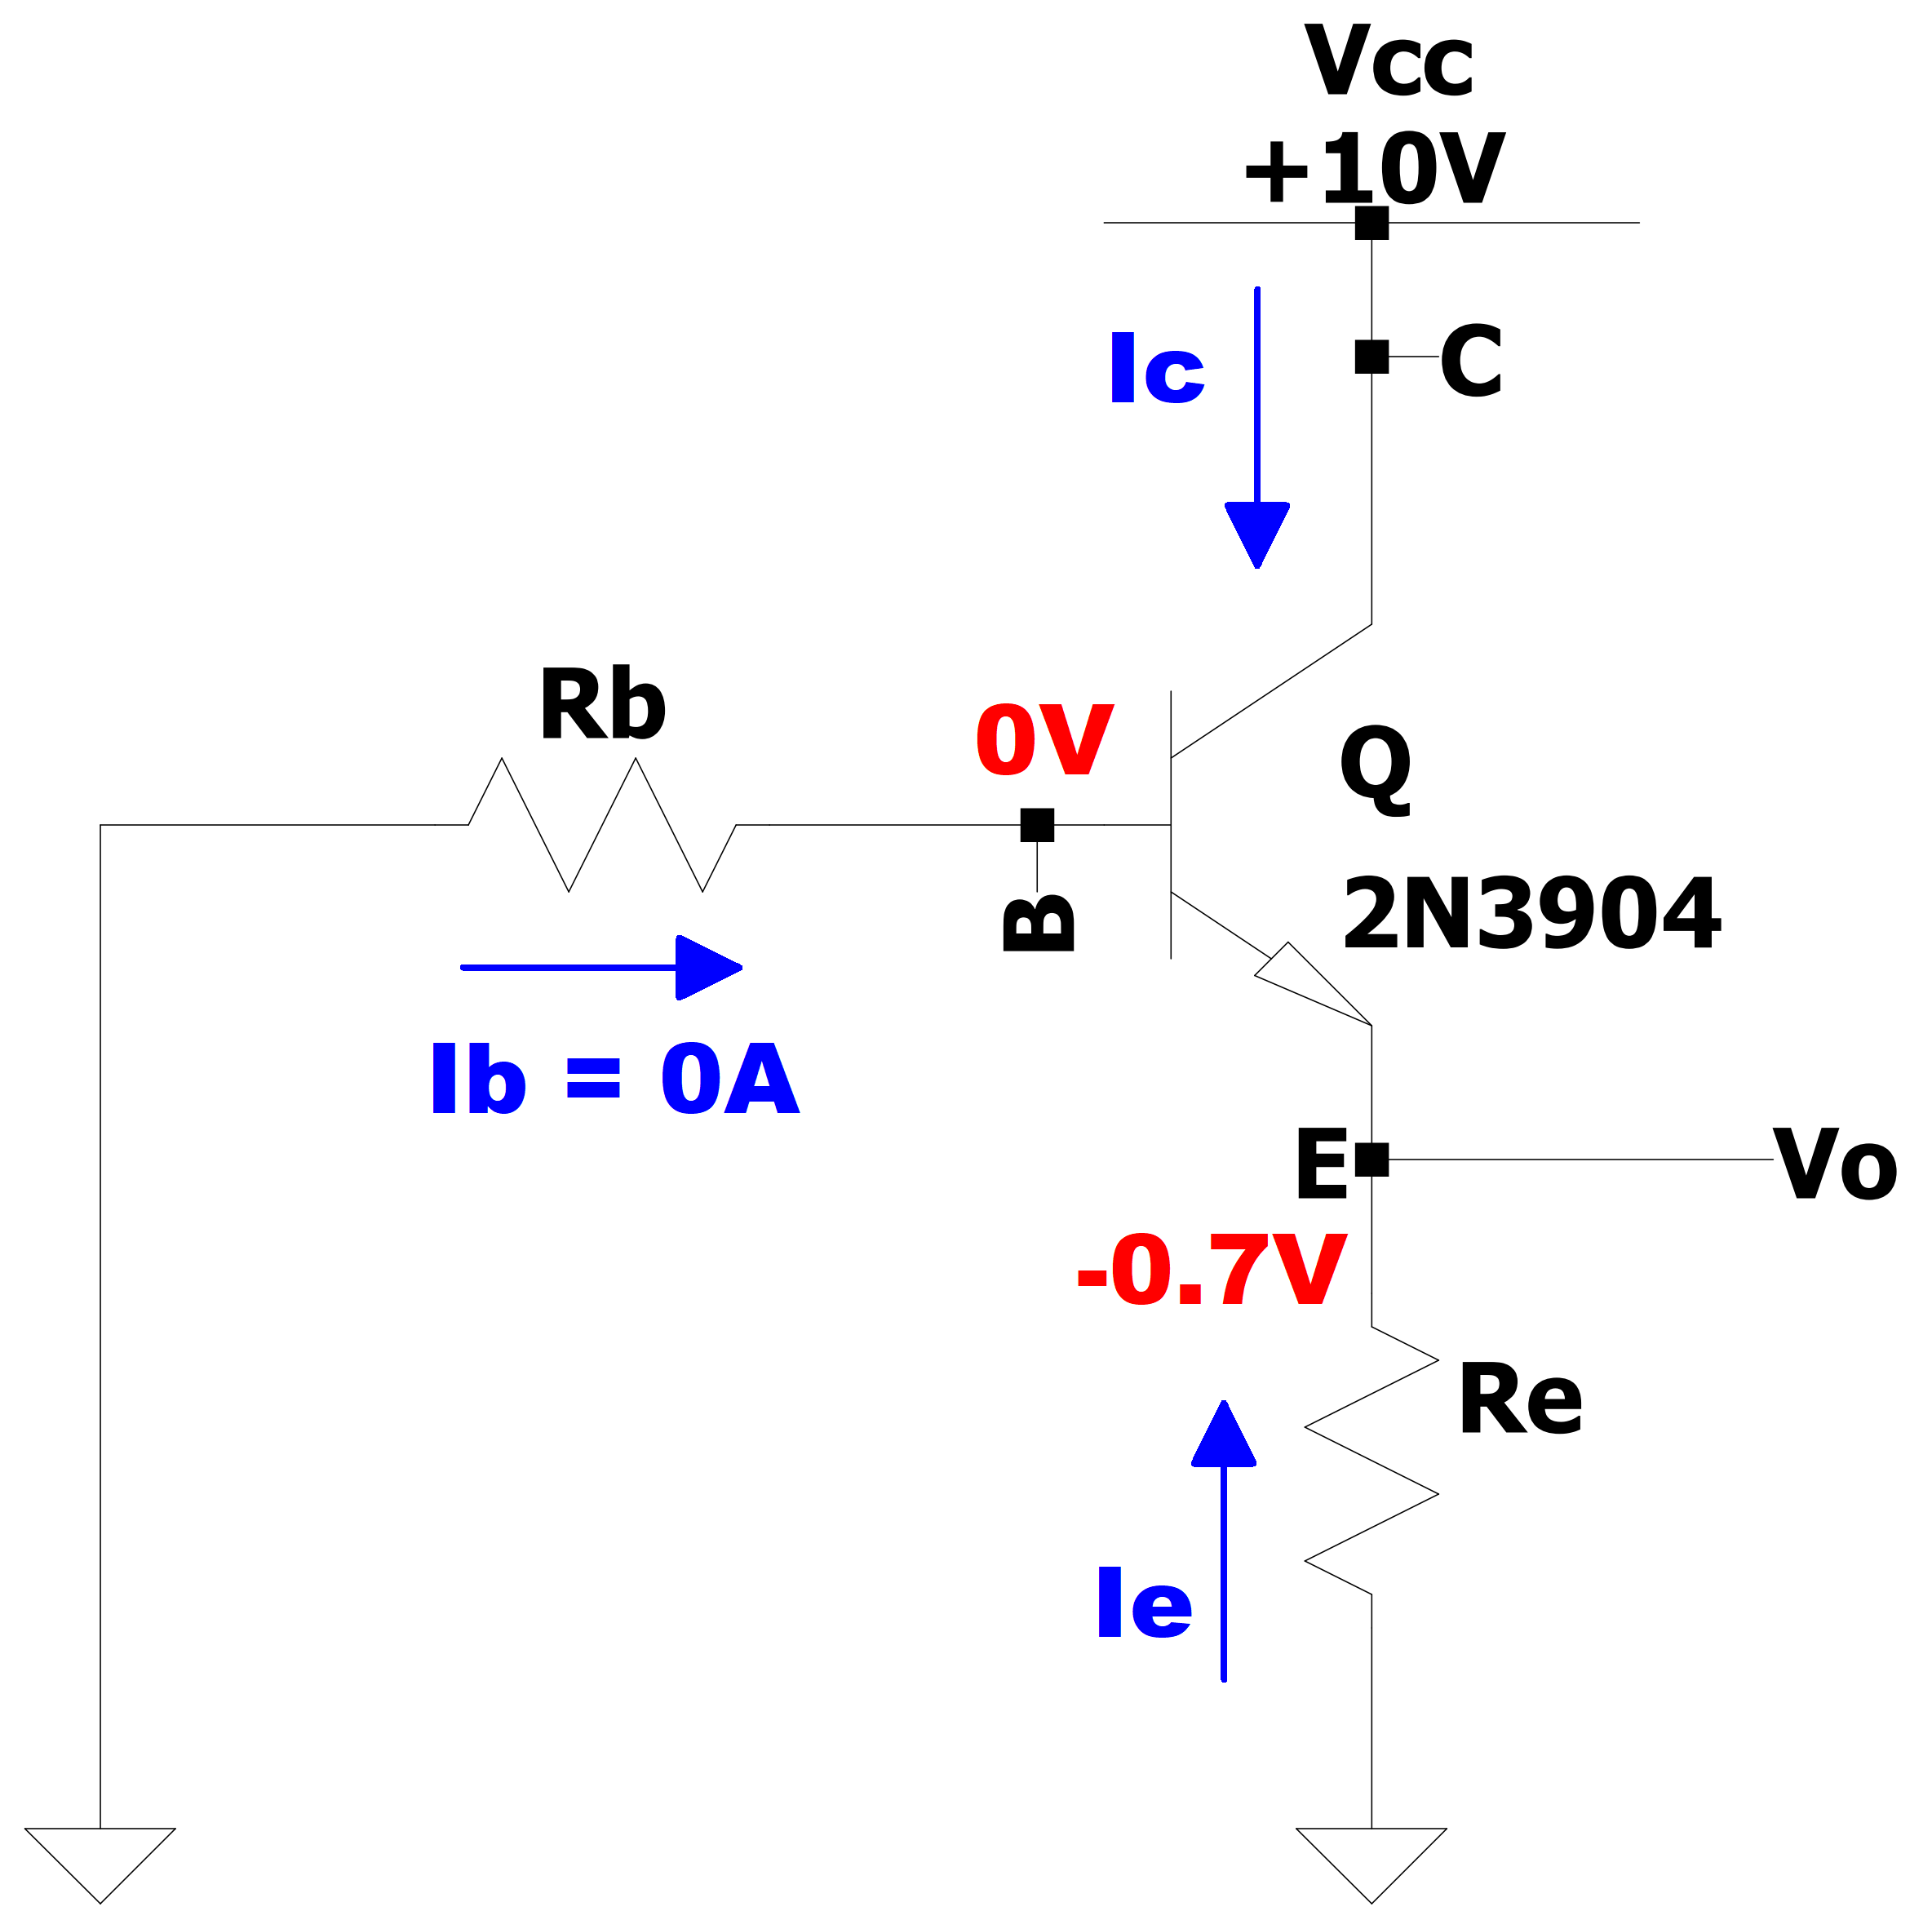
\includegraphics[height=9cm]{immagini/EFv2_1_pl}
\caption{Punto di lavoro dell'\textit{Emitter follower} ad alimentazione singola.}
\label{figura:EFv2_1_pl}
\end{figure}
\\Utilizziamo ancora il modello ideale del transistor, perciò assumiamo che $\displaystyle{\beta\rightarrow\infty}$ e che $I_{B}=0A$. Allora, la corrente che fluisce nella resistenza  $R_B$ è nulla, quindi sarà nulla anche la caduta di tensione ai suoi capi.
\\\indent Suppondendo che il transistor si trovi in regione attiva diretta, la tensione $V_{BE}$ fra la base e l'emettitore è pari a circa +0.7V perché la giunzione è polarizzata direttamente. Dato che sappiamo che $V_{B}=0V$, $V_{E}$ sarà uguale a -0.7V. 
\\\indent La resistenza $R_E$ è attraversata da una corrente che va dalla massa all'emettitore: questo non è possibile, perché implicherebbe che la corrente entri nel transistor e fluisca dall'emettitore al collettore, ovvero nel verso opposto rispetto a quello consentito. Questo porta ad affermare che il transistor non può trovarsi in regione attiva diretta, ma è spento. Finché l'emettitore si trova ad una tensione minore di 0V, ovvero fin quando $V_B$ è minore di 0.7V, il circuito non funzionerà correttamente.
\\\indent Per ovviare a questo problema, bisogna fare in modo che la base del transistor si trovi ad una tensione adeguata. Per alzare il valore di tensione di questo nodo, possiamo sfruttare un partitore di resistenze. Inseriamo allora una resistenza da \SI{130}{k\ohm} fra la tensione di alimentazione e la base del transistor ed un'altra resistenza da \SI{150}{k\ohm} fra la base del transistor e massa. La resistenza di emettitore $R_E$ è invece pari a \SI{7.5}{k\ohm}. Il circuito è mostrato in figura \ref{figura:EFv2_2}.
\begin{figure}[h]
\centering
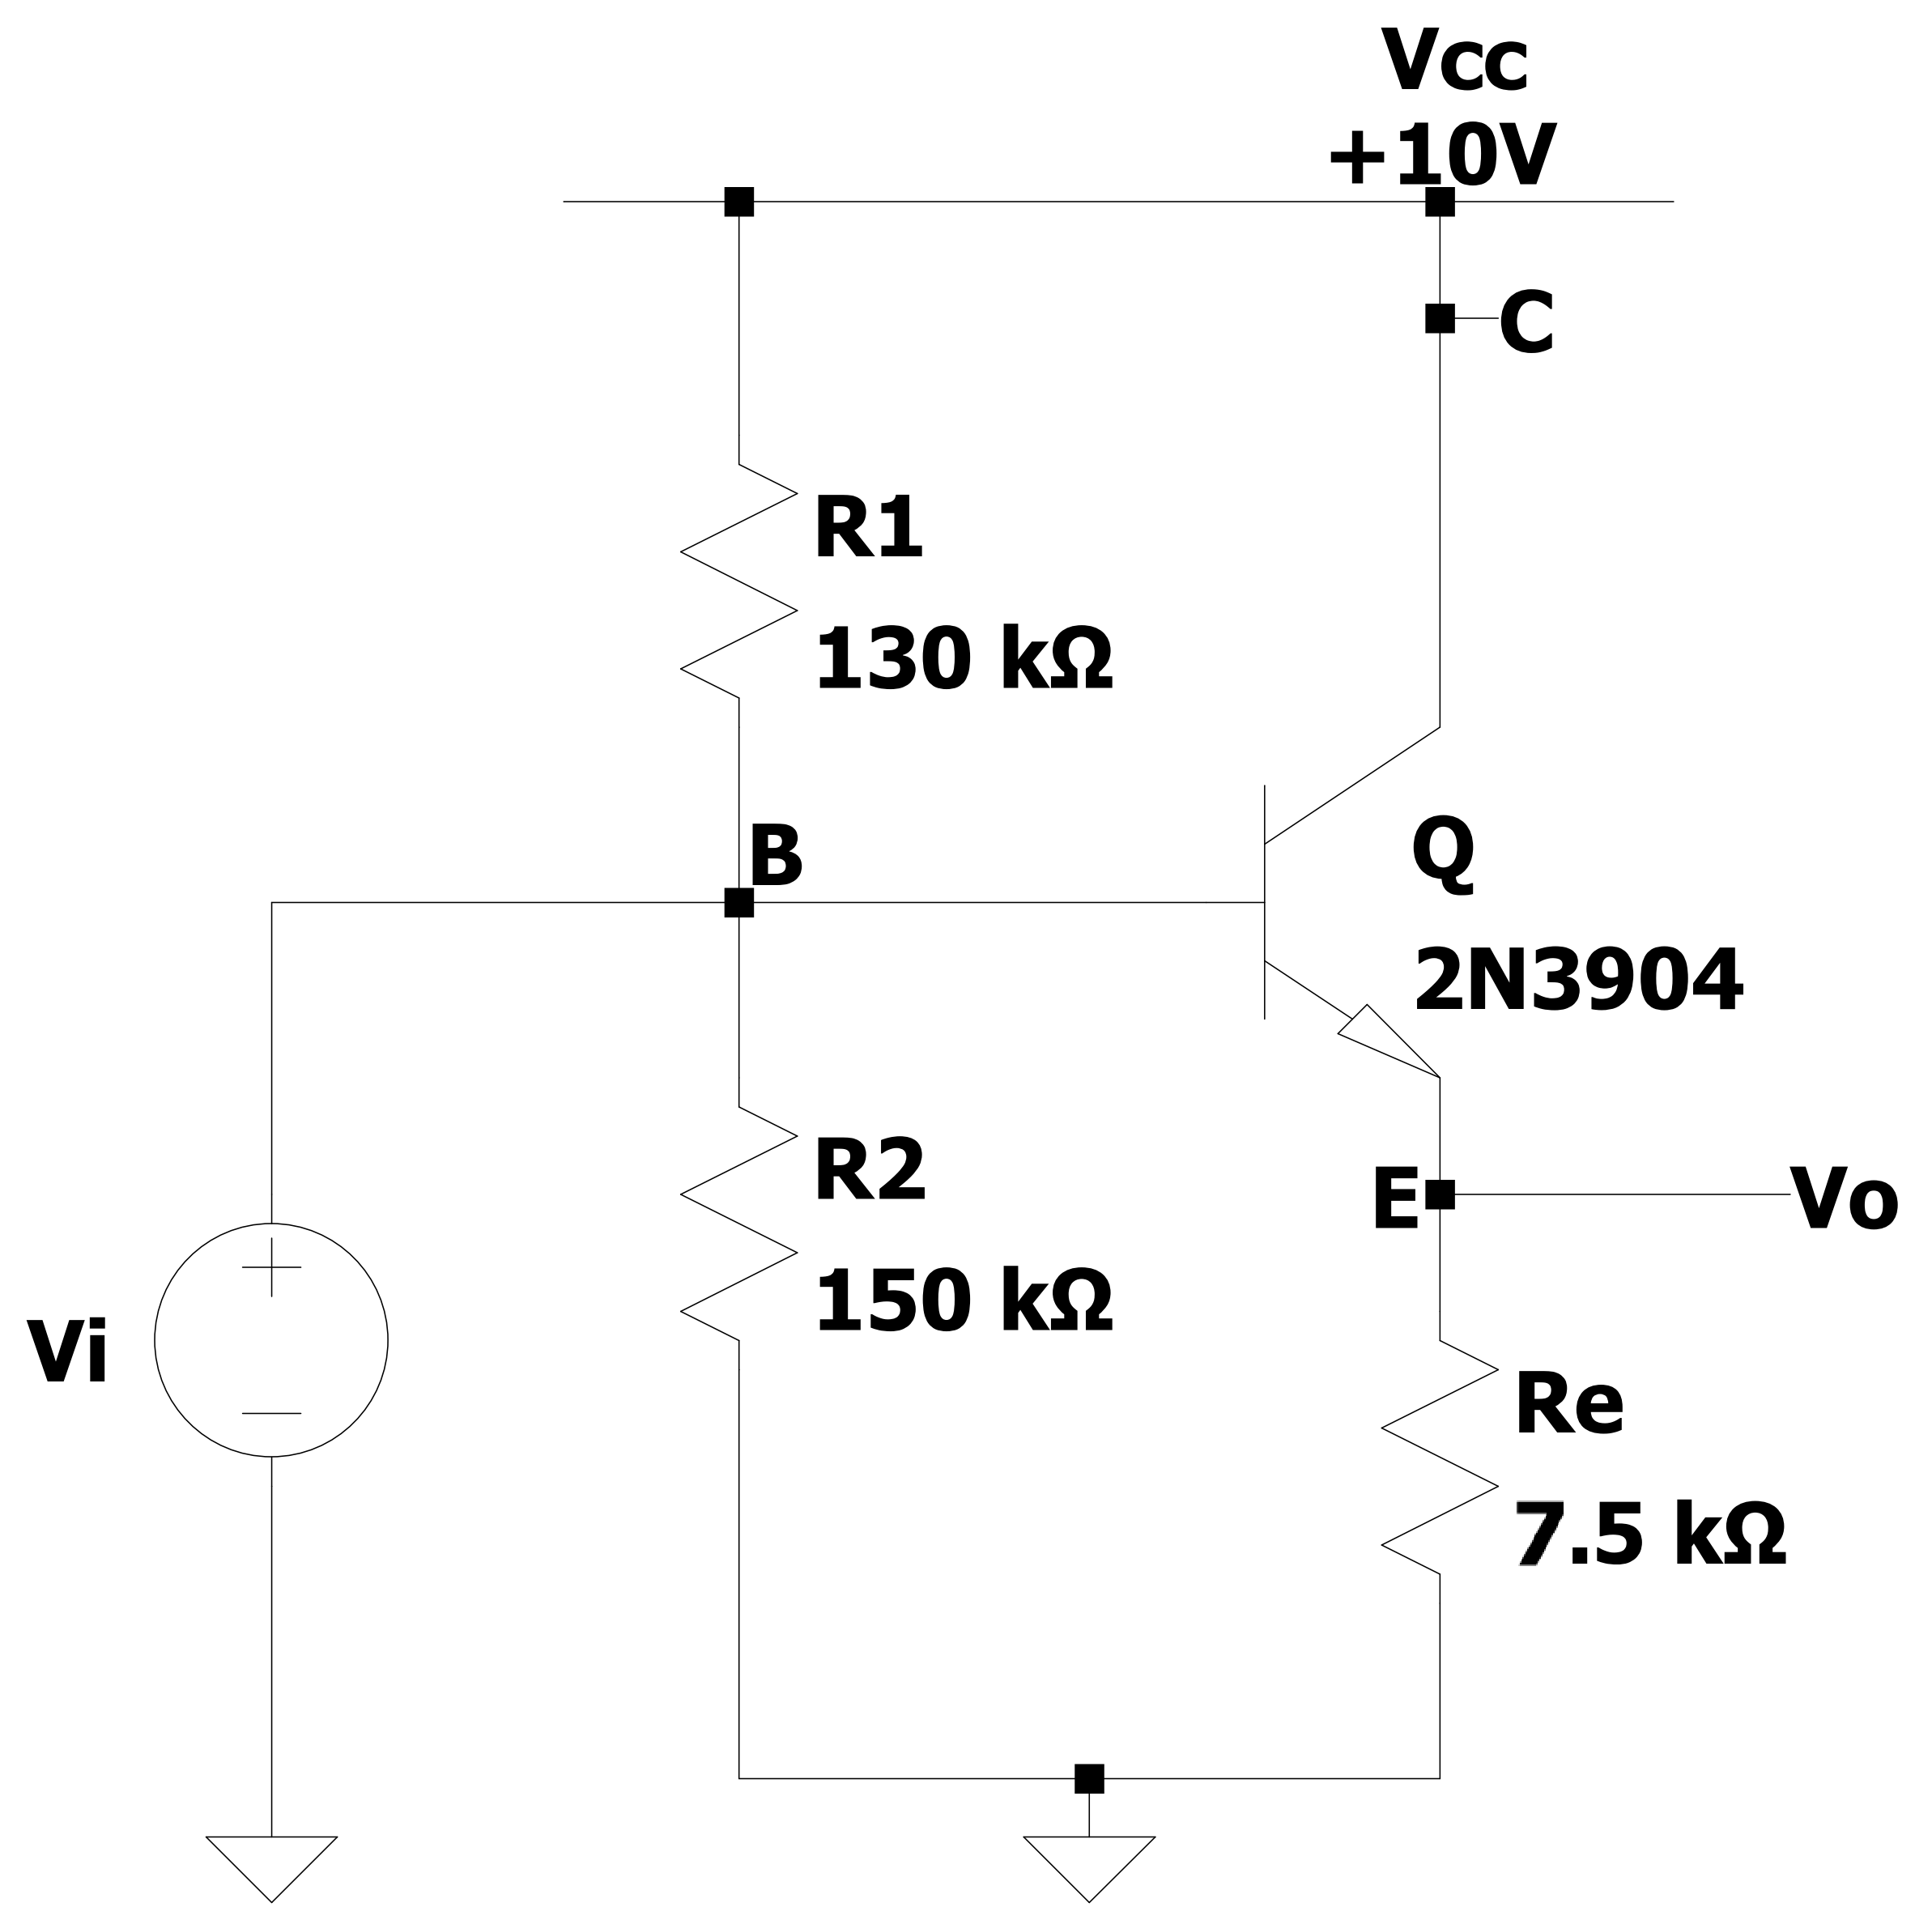
\includegraphics[height=9cm]{immagini/EFv2_2}
\caption{Schema modificato dell'\textit{Emitter follower} ad alimentazione singola.}
\label{figura:EFv2_2}
\end{figure}
\\\indent Ci accorgiamo subito che anche in questo caso il circuito non funziona come dovrebbe, perché sostituendo a $v_i$ un cortocircuito, forziamo ancora la base a massa. Bisogna fare in modo che il generatore di segnale sia disaccoppiato dal circuito in continua, così da evitare che la base venga forzata a massa, ma sia accoppiato in alternata, in modo tale che il segnale applicato in ingresso non venga modificato. Un componente che ha esattamente questo comportamento è il condensatore. \\Proviamo quindi a mettere un condensatore tra il segnale e la base del transistor. Il circuito risultante è la figura \ref{figura:EFv2_3}.
\begin{figure}[h!]
\centering
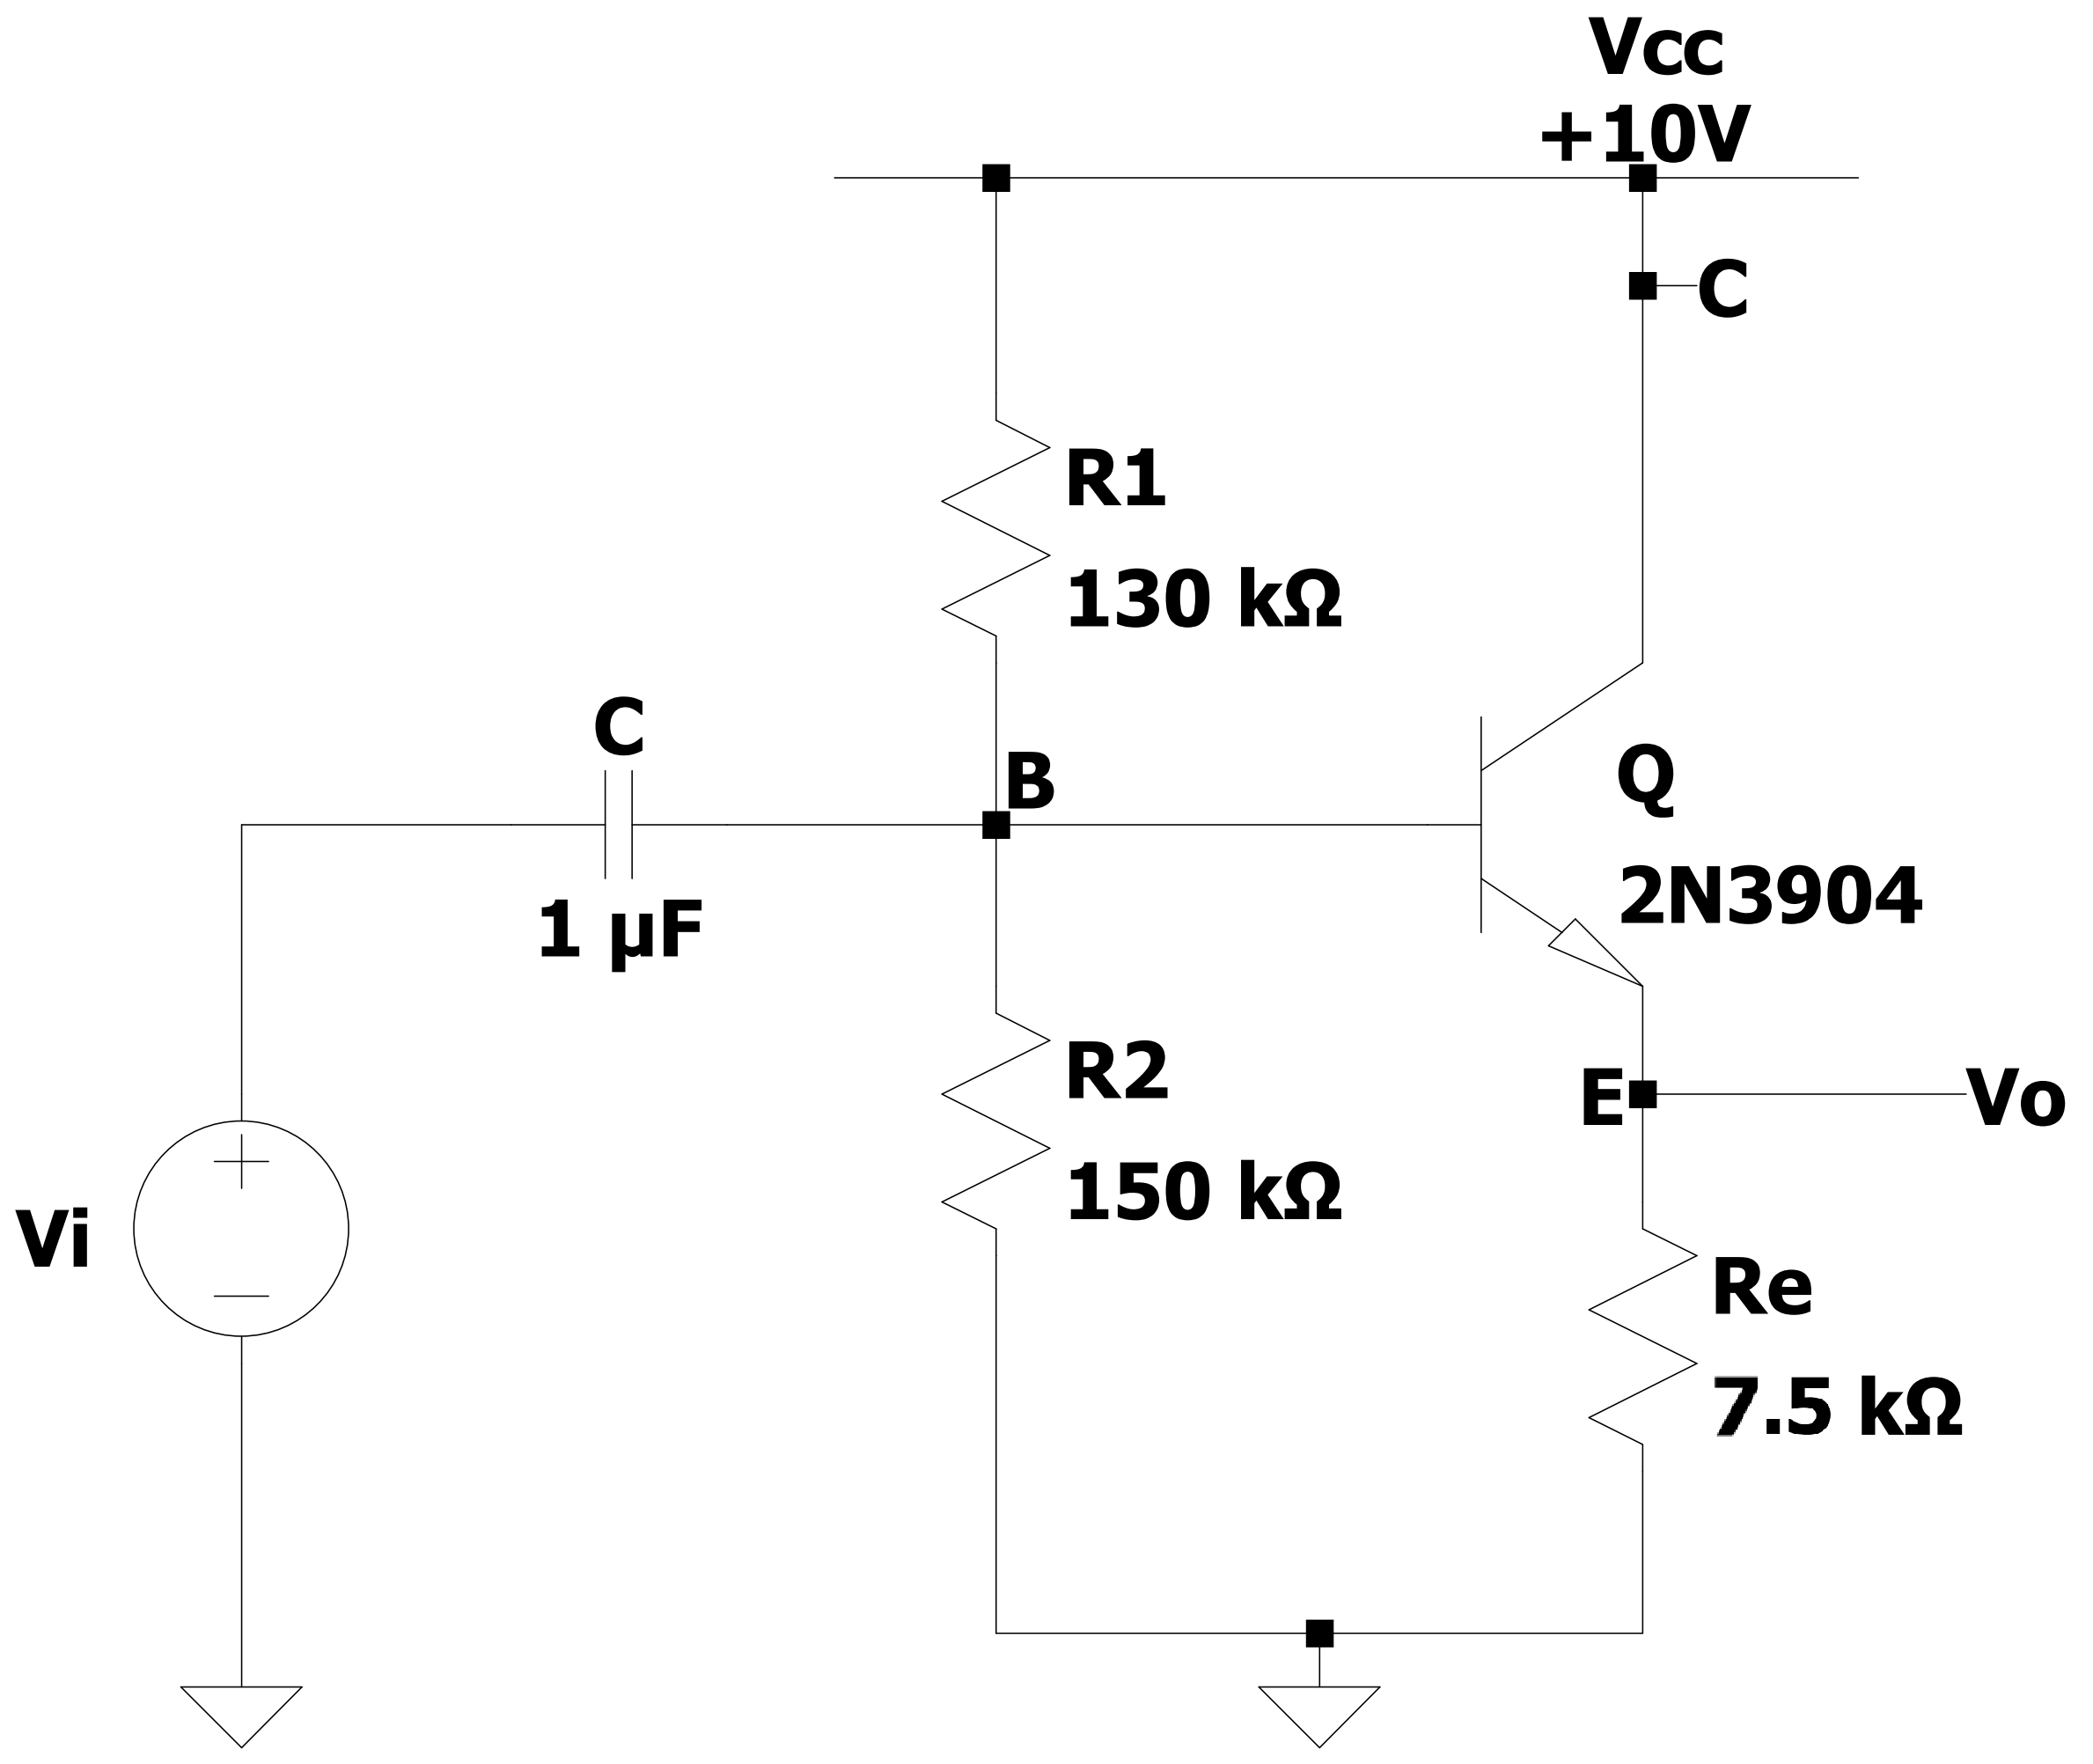
\includegraphics[height=9cm]{immagini/EFv2_3}
\caption{Schema finale dell'\textit{Emitter follower} ad alimentazione singola.}
\label{figura:EFv2_3}
\end{figure}
\\\indent Ora possiamo proseguire l'analisi. Per il punto di lavoro sostituiamo il generatore di segnale con un cortocircuito e il condensatore con un circuito aperto, perciò c'è un circuito aperto fra la massa e la base del transistor, proprio come ci aspettavamo. Lo schema è riportato in figura \ref{figura:EFv2_3_pl}.
\begin{figure}[h]
\centering
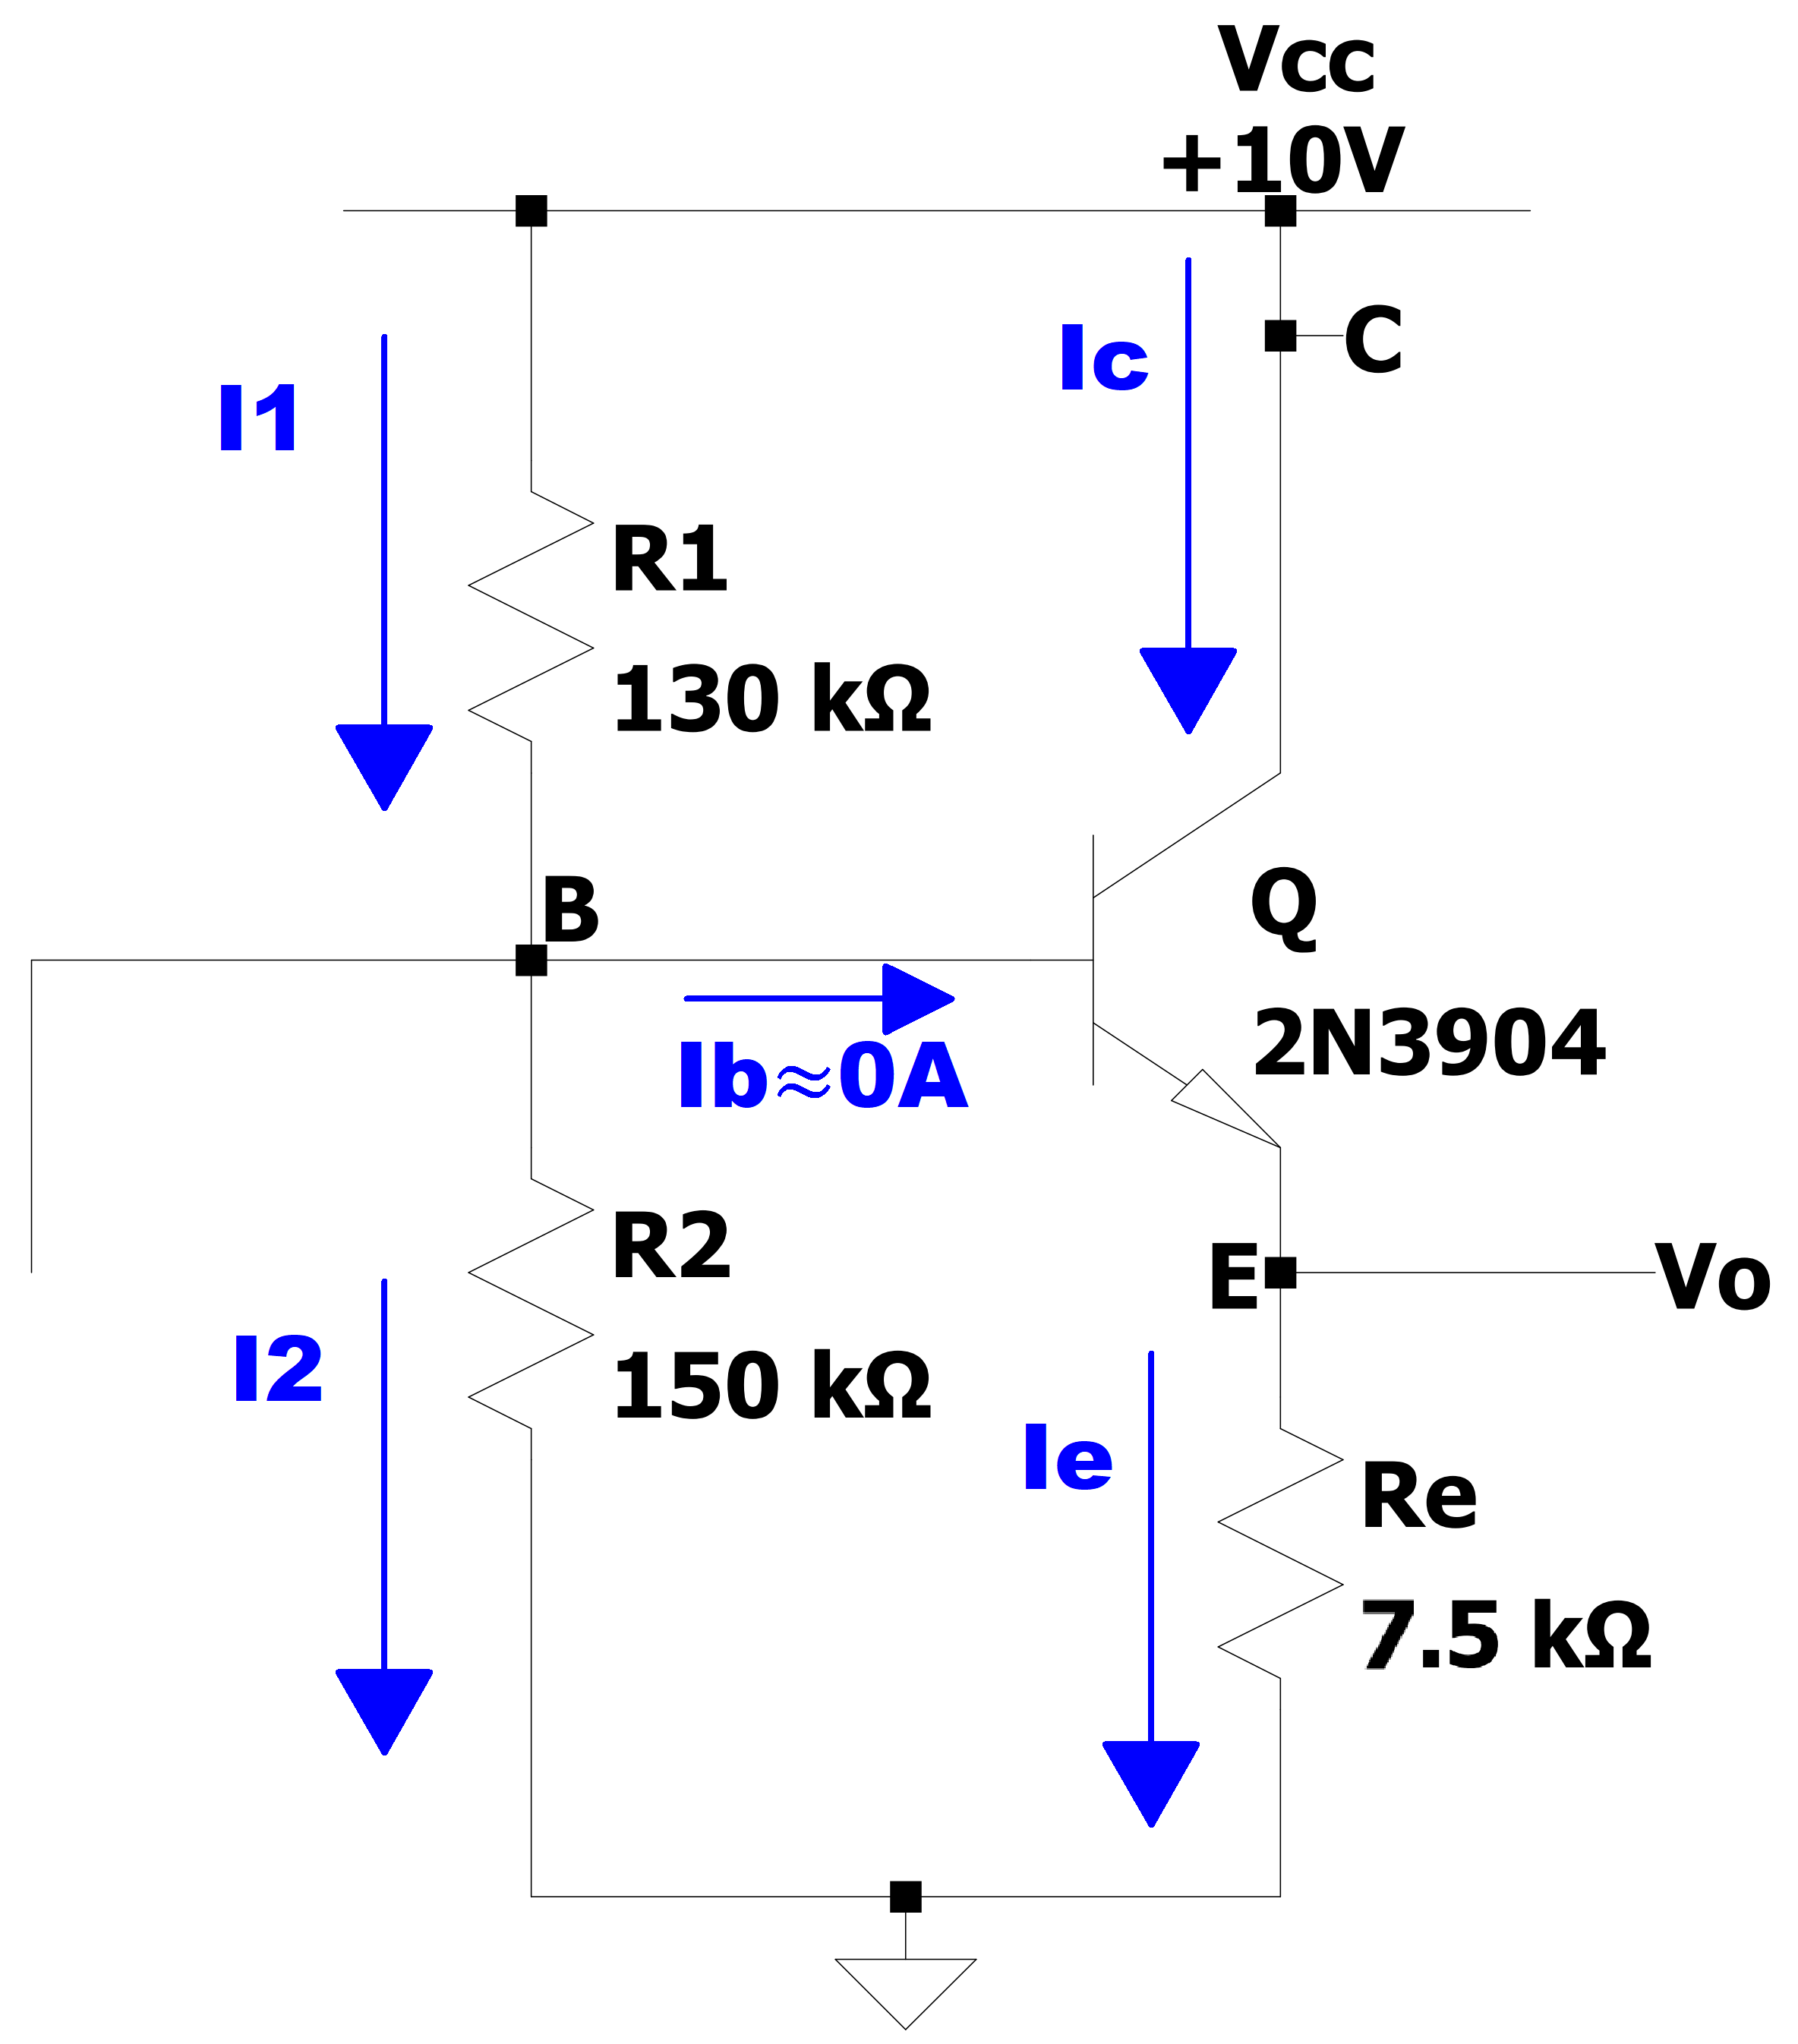
\includegraphics[height=10cm]{immagini/EFv2_3_pl}
\caption{Schema finale del punto di lavoro dell'\textit{Emitter follower} ad alimentazione singola.}
\label{figura:EFv2_3_pl}
\end{figure}
\\Risolviamo il circuito, sempre nell'ipotesi che $\displaystyle{\beta\rightarrow\infty}$ e che quindi $I_{B}=0A$. La tensione $V_B$ può essere ricavata applicando Kirchhoff alla base del transistor, oppure, più semplicemente, si può usare la formula del partitore di tensione:
\\[2pt]\indent$\displaystyle{V_B=\frac{R_2}{R_1+R_2}\cdot 10V=\frac{\SI{150}{k\ohm}}{\SI{280}{k\ohm}}\cdot 10V=5.357V}$
\\[2pt]Dato che $I_B$ è nulla, applicando la legge di Kirchhoff al nodo B otteniamo che $I_1=I_2$, possiamo ricavare una delle due correnti con la legge di Ohm, per esempio calcoliamo $I_2$:
\\[2pt]\indent$\displaystyle{I_2=\frac{V_B-0V}{R_2}=\frac{5.357V}{\SI{150}{k\ohm}}=0.0357mA}$
\\[2pt]Si noti che avremmo ottenuto lo stesso valore se avessimo calcolato $I_1$ al posto che $I_2$.
\\Per calcolare le tensioni e le correnti mancanti si procede esattamente come è stato fatto per l'\textit{Emitter follower} ad alimentazione duale, nella sezione \ref{puntolavoroEFv1}. Bisogna fare attenzione che cambiano i valori delle tensioni e la resistenza $R_E$, perciò saranno diverse anche le correnti che scorrono nei vari rami. 
\\Nella tabella \ref{table:EFv2_3_pl} sono riassunte tutte le grandezze ricavate dal punto di lavoro di questo circuito. 
\begin{table}[h]
	\centering
	\begin{tabular}{|c|c|c|c|c|c|c|c|c|}
		\hline
		\textbf{V\ped{B}[V]} & \textbf{V\ped{C}[V]} & \textbf{V\ped{E}[V]} & \textbf{I\ped{B}[A]} & \textbf{I\ped{1}[mA]} & \textbf{I\ped{2}[mA]} & \textbf{I\ped{E}[mA]} & \textbf{I\ped{C}[mA]} & \textbf{g\ped{m}[A/V]} \\ 
		\hline
		5.357 & 10 & 4.657 & 0 & 0.0357 & 0.0357 & 0.6209 & 0.6209 & 0.024\\ 
		\hline
	\end{tabular}
\caption{Riassunto delle grandezze ricavate dal punto di lavoro del circuito appena discusso.}
\label{table:EFv2_3_pl}
\end{table}
\subsection{Analisi di piccolo segnale}  
Per l'analisi di piccolo segnale consideriamo lo schema di figura \ref{figura:EFv2_3}. Sostituiamo l'alimentazione positiva a 10V con la massa, al posto del transistor utilizziamo il suo modello per piccolo segnale a bassa frequenza ed il condensatore, per ora, non lo sostituiamo con un cortocircuito. Lo schema diventa pertanto quello mostrato in figura \ref{figura:EFv2_3_ps}.
\begin{figure}[h]
\centering
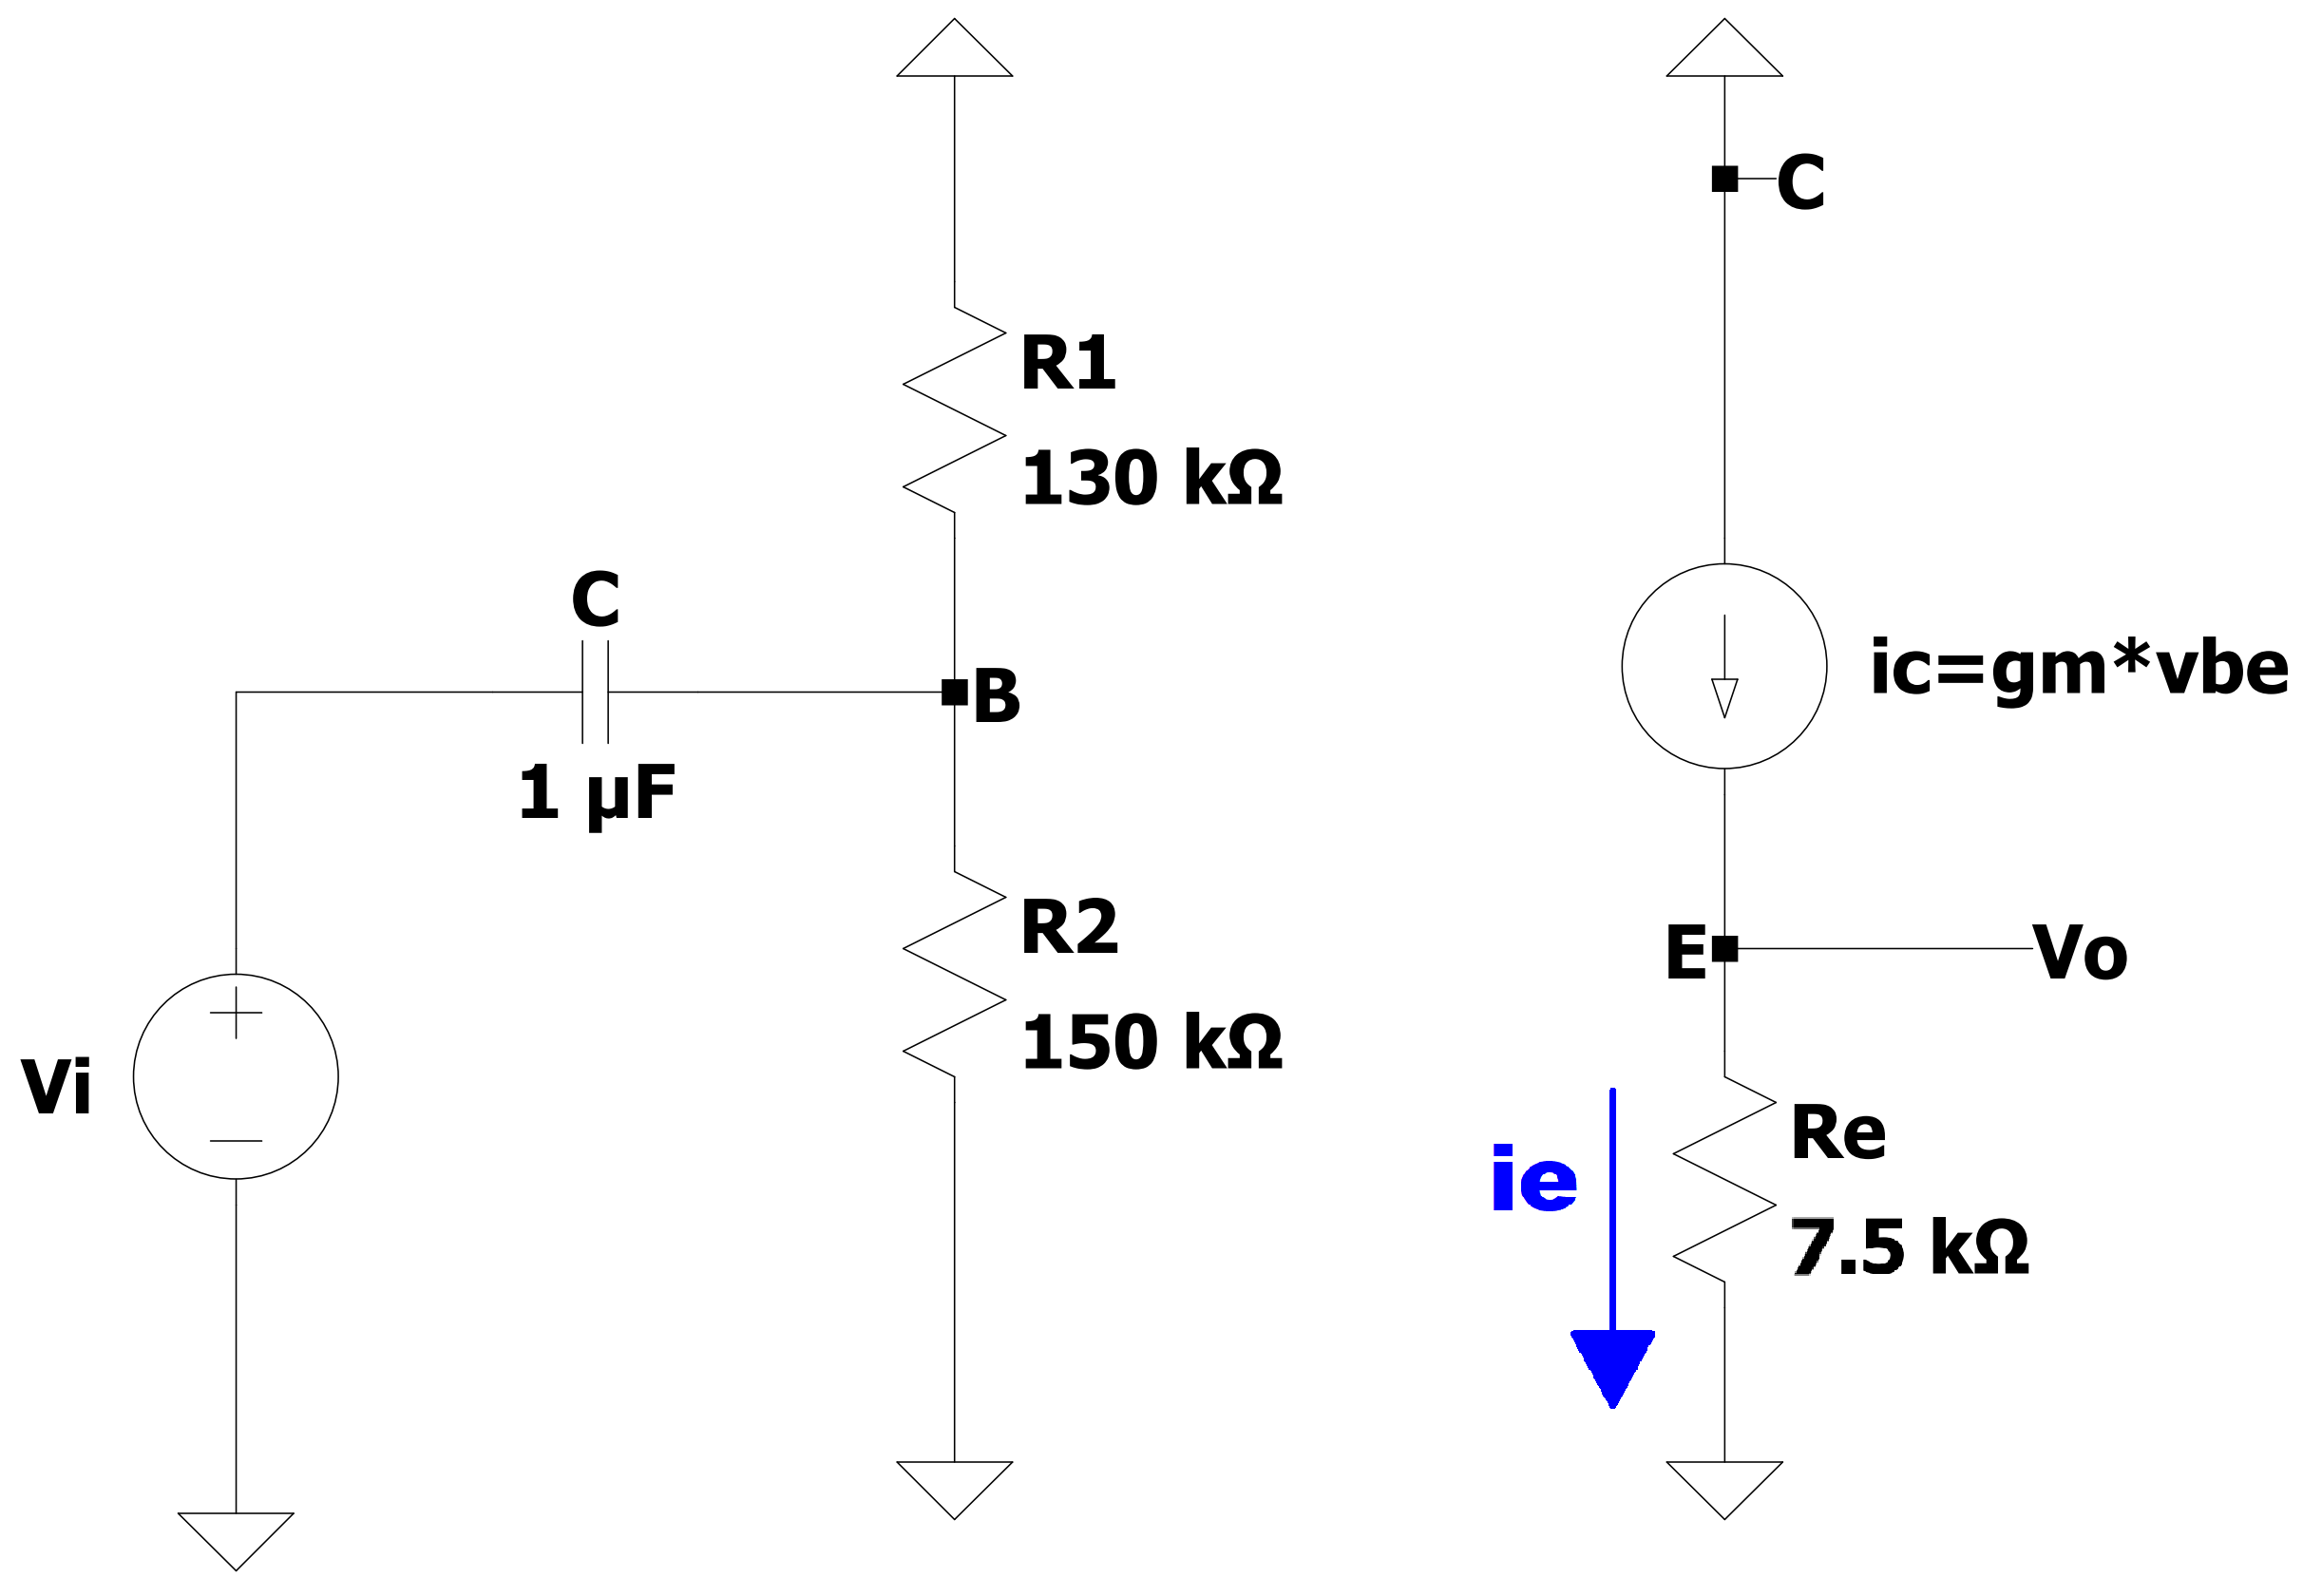
\includegraphics[height=10cm]{immagini/EFv2_3_ps}
\caption{Schema finale dell'analisi di piccolo segnale dell'\textit{Emitter follower} ad alimentazione singola.}
\label{figura:EFv2_3_ps}
\end{figure}
\\Il circuito di destra è identico a quello dell'\textit{Emitter follower} ad alimentazione di duale, cambia solo il valore della resistenza $R_E$. Nel circuito di sinistra possiamo invece riconoscere un filtro passa-alto formato dal condensatore $C$ e dal parallelo fra le resistenze $R_1$ e $R_2$. La frequenza di taglio di questo filtro è:
\\[2pt]\indent $\displaystyle{f_0=\frac{1}{2\pi\cdot C\cdot (R_1\parallelsum R_2)}=\frac{1}{2\pi\cdot 1\mu F\cdot(\SI{130}{k\ohm}\parallelsum\SI{150}{k\ohm})}=\SI{2.285}{\hertz}}$
\\[2pt]Se la frequenza di taglio è sufficientemente bassa, come nel nostro caso, il contributo del filtro passa-alto alla funzione di trasferimento del circuito è trascurabile, pertanto $v_o=v_i$. In caso contrario, nella funzione di trasferimento finale bisogna considerare anche la funzione di trasferimento del filtro.
\subsection{Componenti, strumenti e misure} 
Prima di realizzare la versione finale del circuito \textit{Emitter follower} ad alimentazione singola, abbiamo provato a collegare a massa l'alimentazione negativa del circuito utilizzato prima. In figura \ref{figura:oscillo2} sono riportate la tensione in ingresso e la tensione in uscita al circuito appena modificato. I due segnali sono stati accoppiati in continua.
\begin{figure}[h]
\centering
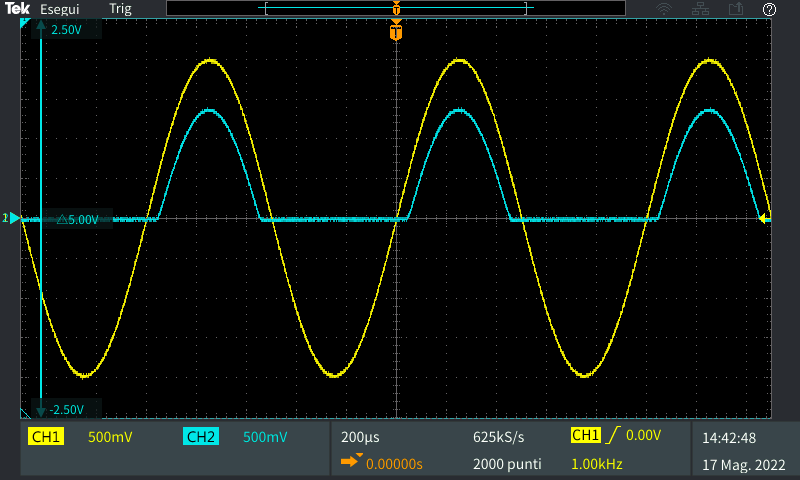
\includegraphics[height=7cm]{immagini/oscillo2}
\caption{Grafico della tensione in ingresso (CH1) e della tensione in uscita (CH2) al circuito.}
\label{figura:oscillo2}
\end{figure}
\\\indent Come ci aspettavamo, il circuito taglia le semionde negative: quando il segnale in ingresso è minore di 0.7V, la tensione in uscita rimane a 0V. Dal grafico possiamo anche vedere che la caduta di tensione data dalla giunzione p-n fra base ed emettitore rimane.
\\\indent Dopo aver verificato che il circuito si comporta come ci aspettavamo dall'analisi teorica, abbiamo costruito la versione finale già illustrata in figura \ref{figura:EFv2_3}. Il circuito, di cui si riporta la fotografia (figura \ref{figura:fotoEFv2_3}), è stato realizzato su una breadboard utilizzando questi componenti:
\begin{itemize}
\item transistor bipolare NPN 2N3904;
\item due resistenze connesse in serie, $R_{E_1}$ e $R_{E_2}$, entrambe da \SI{3.9}{k\ohm}, per realizzare la resistenza $R_E$ da \SI{7.8}{k\ohm};
%% da QUI
\item due resistenze, una da \SI{82}{k\ohm} ($R_{11}$) ed una da \SI{39}{k\ohm} ($R_{12}$) connesse in serie, per realizzare la resistenza $R_1$ da \SI{120}{k\ohm}.
\item tre resistenze, una da \SI{39}{k\ohm} ($R_{21}$), una da \SI{27}{k\ohm} ($R_{22}$) ed una da \SI{82}{k\ohm} ($R_{23}$) connesse in serie, per realizzare la resistenza $R_2$ da \SI{148}{k\ohm}.
\item un condensatore da \SI{1}{\mu\farad}
\end{itemize}
Per quanto riguarda $R_E$, non è stato possibile utilizzare una resistenza del valore indicato (\SI{7.5}{k\ohm}), ma con queste connessioni otteniamo una resistenza di valore poco maggiore (solo il 4\%). Lo stesso discorso vale per le altre due resistenze, però quello che conta in questo caso non è tanto il valore del singolo componente, quanto il fattore di partizione. Il fattore di partizione che dovremmo ottenere è di 0.5357, quello che otteniamo è di 0.5522, ovvero solo il 3\% in più.
\begin{figure}[h]
\centering
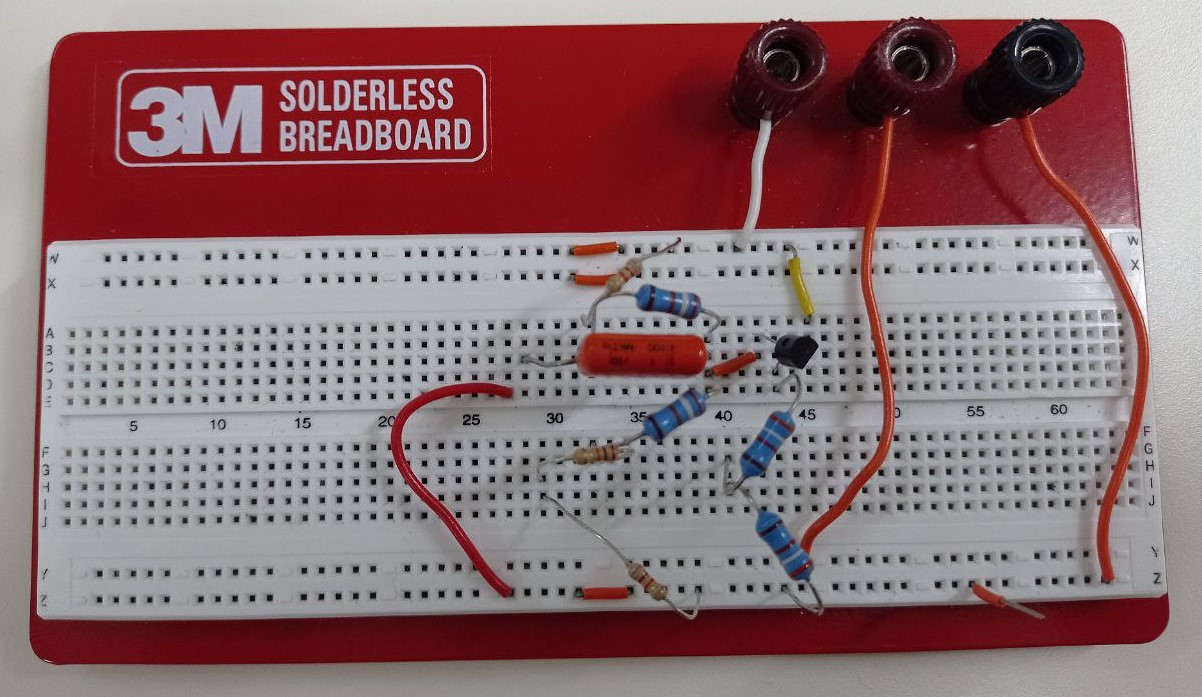
\includegraphics[height=6.6cm]{immagini/fotoEFv2_3}
\caption{Fotografia del circuito \textit{Emitter follower} ad alimentazione singola realizzato in laboratorio.}
\label{figura:fotoEFv2_3}
\end{figure}
\\Per le misure e le analisi, sono stati utilizzati i seguenti strumenti:
\begin{itemize}
\item alimentatore da banco, con alimentazione positiva impostata a 10V e limite in corrente di 50mA;
\item generatore di forme d'onda;
\item multimetro da banco;
\item oscilloscopio a due canali.
\end{itemize}
Come per il circuito precedente, per prima cosa andiamo a misurare il valore delle resistenze con il multimetro. I valori ottenuti sono mostrati in tabella \ref{table:EFv2_3_comp}.
\\
\begin{table}[h]
	\centering
	\begin{tabular}{|c|c|c|}
	\cline{2-3} 
	\multicolumn{1}{c|}{} & \textbf{Valore nominale} & \textbf{Valore misurato}\\ 
		%\hline
		%{} & \textbf{Valore nominale} & \textbf{Valore misurato} \\ 
		\hline
		$\mathbf{R_{E_1}}$& \SI{3.9}{k\ohm} & \SI{3.88}{k\ohm} \\ 
		\hline
		$\mathbf{R_{E_2}}$& \SI{3.9}{k\ohm} & \SI{3.91}{k\ohm} \\ 
		\hline
		$\mathbf{R_{11}}$& \SI{82}{k\ohm} & \SI{82.67}{k\ohm} \\ 
		\hline
		$\mathbf{R_{12}}$& \SI{39}{k\ohm} & \SI{38.86}{k\ohm} \\ 
		\hline
		$\mathbf{R_{21}}$& \SI{39}{k\ohm} & \SI{38.80}{k\ohm} \\ 
		\hline
		$\mathbf{R_{22}}$& \SI{27}{k\ohm} & \SI{26.87}{k\ohm} \\ %CONTROLLA VALORE
		\hline
		$\mathbf{R_{23}}$& \SI{82}{k\ohm} & \SI{82.18}{k\ohm} \\ 
		\hline
	\end{tabular}
\caption{Grandezze misurate prima di realizzare il circuito.}
\label{table:EFv2_3_comp}
\end{table}
\\I valori delle resistenze saranno quindi $R_E=\SI{7.79}{k\ohm}$, $R_1=\SI{121.53}{k\ohm}$ e $R_2=\SI{147.85}{k\ohm}$. Ora studiamo il punto di lavoro del circuito. Misuriamo le tensioni dei nodi B ed E con il multimetro e calcoliamo le correnti $I_1$, $I_2$ e $I_E$ con la legge di Ohm. Ricaviamo quindi per differenza, applicando la legge di Kirchhoff, le correnti $I_B$ e $I_C$:
\\[2pt]\indent $\displaystyle{I_1=I_B+I_2\rightarrow I_B=I_1-I_2}$
\\\indent $\displaystyle{I_E=I_C+I_B\rightarrow I_C=I_E-I_B}$
\\[2pt]Tutti i valori misurati sono riportati in tabella \ref{table:EFv2_3_pl_mis}. Anche in questo caso le misure sono molto vicine ai valori teorici.
\begin{table}[h]
	\centering
	\begin{tabular}{|c|c|c|c|c|c|c|c|c|}
		\hline
		\textbf{V\ped{B}[V]} & \textbf{V\ped{C}[V]} & \textbf{V\ped{E}[V]} & \textbf{I\ped{1}[\textmu A]} & \textbf{I\ped{2}[\textmu A]} & \textbf{I\ped{E}[\textmu A]} & \textbf{I\ped{B}[\textmu A]} & \textbf{I\ped{C}[\textmu A]} & \textbf{g\ped{m}[A/V]} \\ 
		\hline
		5.228 & 10.000 & 4.607 & 39.27 & 35.36 & 591.40 & 3.91 & 587.49 & 0.023\\ 
		\hline
	\end{tabular}
\caption{Grandezze misurate dallo studio del punto di lavoro del circuito.}
\label{table:EFv2_3_pl_mis}
\end{table}
\\Terminato lo studio del punto di lavoro, applichiamo il segnale al circuito collegando il generatore di forme d'onda e osserviamo il grafico della tensione in ingresso e della tensione in uscita con l'oscilloscopio. La forma d'onda utilizzata è una sinusoide di frequenza $f=\SI{1}{k\hertz}$ e tensione picco-picco $V_{PP}$ di 2V. Il grafico è riportato in figura \ref{figura:oscillo3}, i due segnali sono accoppiati in continua.
\begin{figure}[h]
\centering
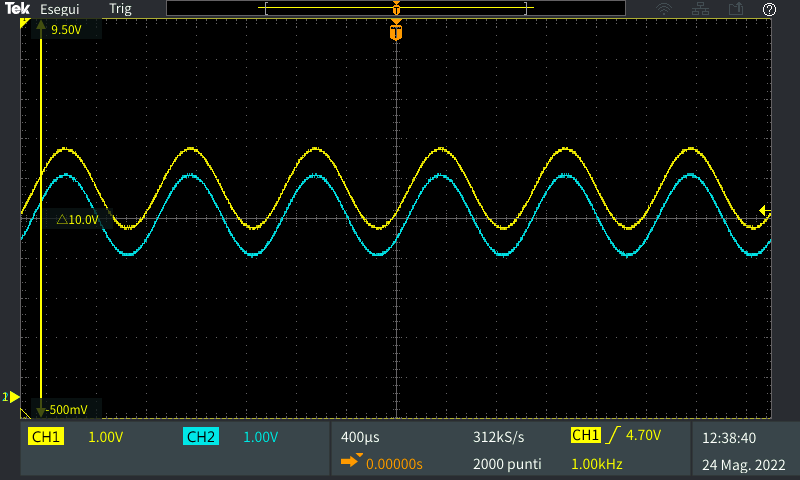
\includegraphics[height=7cm]{immagini/oscillo3}
\caption{Grafico della tensione in ingresso (CH1) e della tensione in uscita (CH2) al circuito.}
\label{figura:oscillo3}
\end{figure}
\\Dal grafico possiamo vedere che il guadagno del circuito è unitario perché entrambe le sinusoidi hanno la stessa ampiezza. La tensione applicata in ingresso, analogamente all'\textit{Emitter follower} ad alimentazione duale, la ritroviamo in uscita con una differenza di circa 0.7V, che è la caduta di tensione data dalla giunzione p-n fra base ed emettitore. I segnali di tensione in ingresso e in uscita sono in fase. 
%----------------------------------------------------------------------------------------
%	CIRCUITO 2: COMMON EMITTER AMPLIFIER
%----------------------------------------------------------------------------------------
\clearpage
\newpage
\chapter{Circuito 2: Common Emitter Amplifier}
\section{Introduzione} 
\section{Prima versione} % senza degenerazione emitter, solo trattazione teorica non realizzato in lab
\subsection{Schema} %?mettere
\subsection{Analisi del circuito} 
\section{Seconda versione} % con degenerazione emitter, alimentazione duale
\subsection{Punto di lavoro} 
\subsection{Analisi di piccolo segnale} 
\subsection{Componenti, strumenti e misure} 
\section{Terza versione} % con degenerazione emitter, alimentazione singola (in piccolo segnale aggiungi già il condensatore)
\subsection{Punto di lavoro} 
\subsection{Analisi di piccolo segnale}  
\subsection{Componenti, strumenti e misure} 


%----------------------------------------------------------------------------------------
%	CIRCUITI 3 E 4: AMPLIFICATORE OPERAZIONALE \mu A741
%----------------------------------------------------------------------------------------
\clearpage
\newpage
\chapter{Circuiti 3 e 4: Amplificatore operazionale \textmu A741}
\section{Introduzione} 
\section{Amplificatore invertente} 
\subsection{Schema} %?mettere
\subsection{Analisi del circuito} 
\subsection{Componenti, strumenti e misure} 
\section{Integratore} 
\subsection{Schema} %?mettere
\subsection{Analisi del circuito} 
\subsection{Componenti, strumenti e misure} 





%----------------------------------------------------------------------------------------

\end{document}
